% ============================================================
%  CHAPITRE 9 : Résultats de la simulation et interprétation
% ============================================================
\chapter{Résultats de la simulation et interprétation}
\label{chap:resultats_simulation}

\section{Introduction}
\label{sec:intro_resultats}

Ce chapitre présente et analyse les résultats des simulations numériques OpenFOAM réalisées pour les trois débits laminés retenus : $Q_{10} = 160{,}74$ m³/s, $Q_{100} = 507{,}54$ m³/s et $Q_{1\,000} = 794{,}93$ m³/s. Pour chaque débit, les résultats sont présentés dans l'ordre suivant :
\begin{enumerate}
    \item \textbf{Champ de vitesse} : profil de la vitesse le long de l'évacuateur et graphe de l'évolution des valeurs exactes ;
    \item \textbf{Champ de pression} : profil de la pression le long de l'évacuateur et graphe des valeurs exactes ;
    \item \textbf{Hauteur d'eau} : visualisation de la lame d'eau aux trois points caractéristiques de l'ouvrage (seuil, coursier, cuillère) ;
    \item \textbf{Jet et point d'impact} : trajectoire du jet en aval de la cuillère et coordonnées du point d'impact.
\end{enumerate}

Toutes les visualisations sont réalisées sous ParaView \cite{ayachit2015paraview} à partir des champs \texttt{U}, \texttt{p\_rgh} et \texttt{alpha.water} extraits en régime quasi-permanent.

% ============================================================
%  SECTION 9.1 : Q10
% ============================================================
\section{Résultats pour le débit décennal $Q_{10} = 160{,}74$ m³/s}
\label{sec:resultats_q10}

\subsection{Champ de vitesse}
\label{subsec:q10_vitesse}

La figure \ref{fig:q10_U_profil} présente le profil de la vitesse $\|\mathbf{U}\|$ le long de l'évacuateur de crues dans le plan médian longitudinal, pour le débit décennal $Q_{10}$.

\begin{figure}[H]
    \centering
    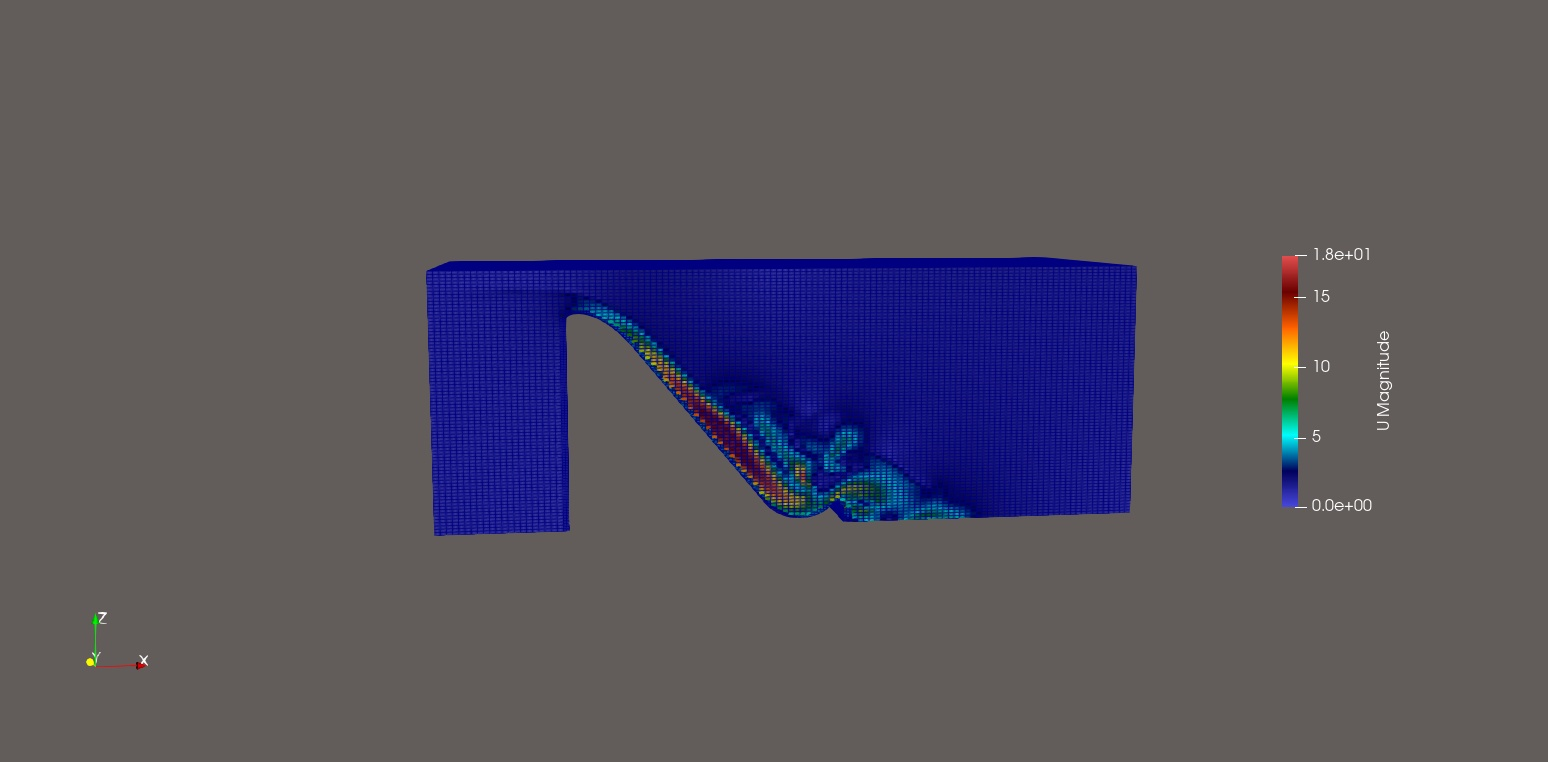
\includegraphics[width=\textwidth]{figures/ch9_q10_U_profil.jpeg}
    \caption{Profil du champ de vitesse $\|\mathbf{U}\|$ (m/s) le long de l'évacuateur de crues — débit décennal $Q_{10} = 160{,}74$ m³/s. L'écoulement s'accélère progressivement depuis la retenue jusqu'à la cuillère, où la vitesse atteint son maximum.}
    \label{fig:q10_U_profil}
\end{figure}

Le profil de vitesse montre une accélération progressive de l'écoulement depuis la zone de retenue (vitesses quasi nulles) jusqu'à la crête du seuil Creager, puis le long du coursier où l'écoulement devient nettement torrentiel. Les vitesses maximales sont atteintes à la sortie de la cuillère saut de ski. Le gradient de vitesse au voisinage des parois traduit bien le développement de la couche limite turbulente, correctement représenté par le modèle $k$-$\omega$ SST.

La figure \ref{fig:q10_U_graphe} présente l'évolution quantitative de la vitesse le long de l'axe longitudinal de l'évacuateur.

\begin{figure}[H]
    \centering
    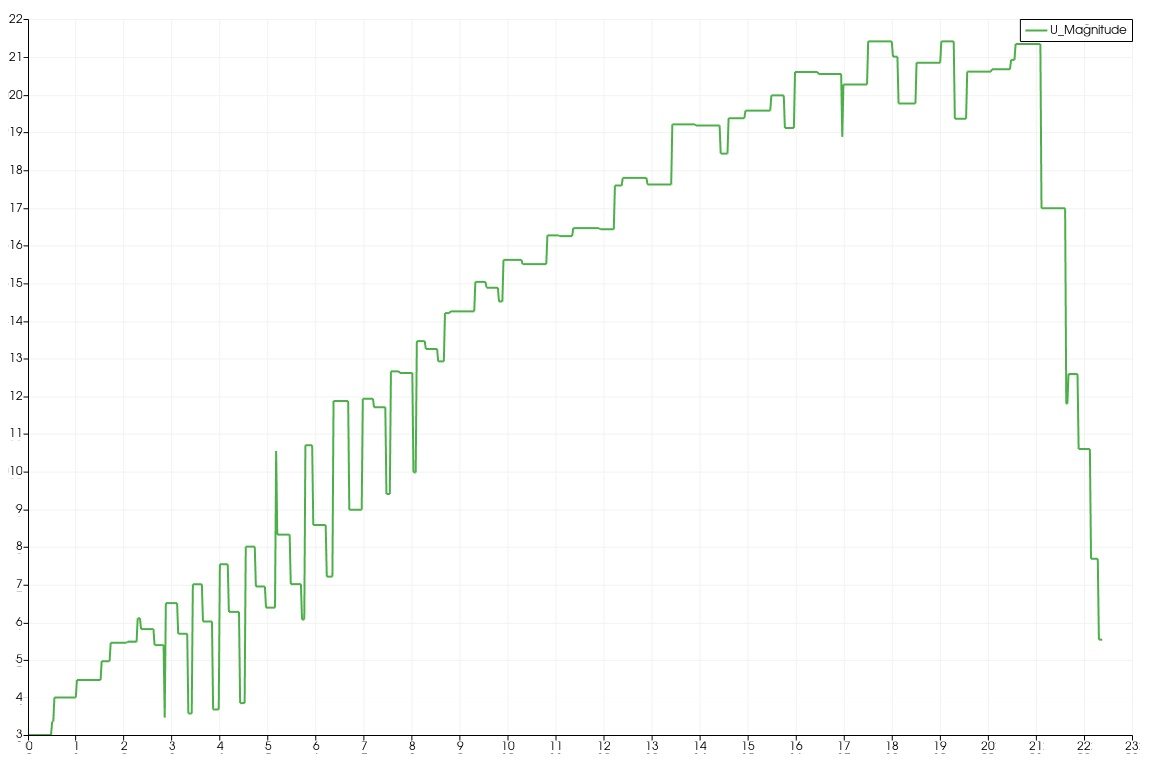
\includegraphics[width=\textwidth]{figures/ch9_q10_U_graphe.jpeg}
    \caption{Évolution de la vitesse $\|\mathbf{U}\|$ (m/s) le long de l'axe longitudinal de l'évacuateur — débit décennal $Q_{10} = 160{,}74$ m³/s. Les coordonnées curvilignes permettent de localiser précisément les zones d'accélération sur le seuil et le coursier.}
    \label{fig:q10_U_graphe}
\end{figure}

Le graphe confirme la montée monotone de la vitesse le long du coursier, caractéristique d'un écoulement supercritique en canal à forte pente. Les valeurs numériques obtenues sont cohérentes avec les résultats théoriques de la méthode des pas du chapitre \ref{chap:dimensionnement_theorique}.

\subsection{Champ de pression}
\label{subsec:q10_pression}

La figure \ref{fig:q10_P_profil} présente la distribution de la pression $p$ le long de l'évacuateur pour le débit décennal.

\begin{figure}[H]
    \centering
    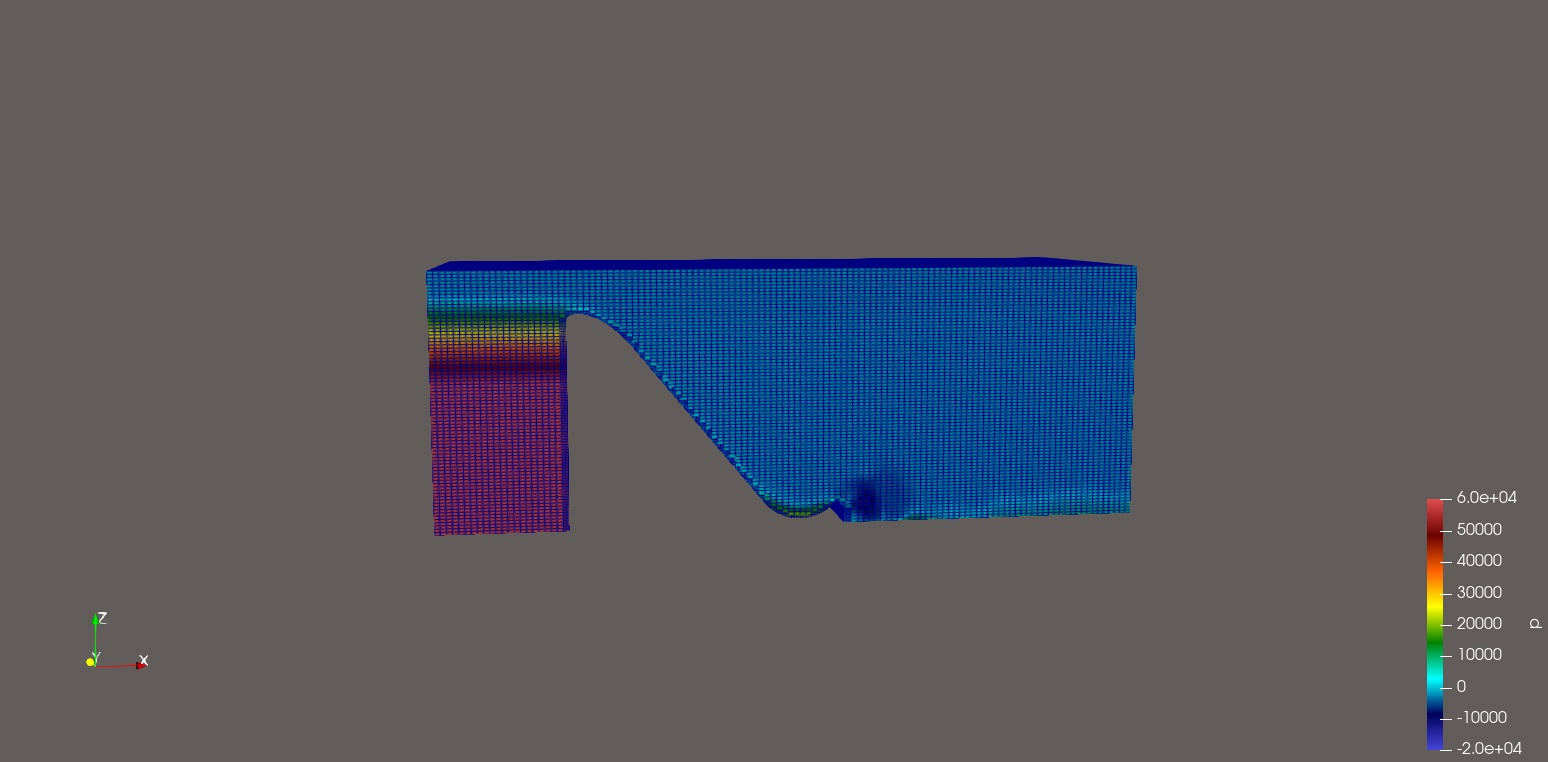
\includegraphics[width=\textwidth]{figures/ch9_q10_P_profil.jpeg}
    \caption{Profil du champ de pression $p$ (Pa) le long de l'évacuateur de crues — débit décennal $Q_{10} = 160{,}74$ m³/s. La pression est maximale dans la retenue amont (hydrostatique) et décroît le long du coursier ; une surpression locale est visible au niveau de la cuillère saut de ski.}
    \label{fig:q10_P_profil}
\end{figure}

Le profil de pression est dominé par la distribution hydrostatique dans la retenue amont. Le long du coursier, la pression diminue conformément à l'augmentation de vitesse (conservation de l'énergie). La courbure convexe de la cuillère saut de ski génère une surpression locale sur le radier, due à l'effet centrifuge de la déviation du jet — phénomène attendu et compatible avec la géométrie dimensionnée à la section \ref{sec:geometrie_cuillere}.

\begin{figure}[H]
    \centering
    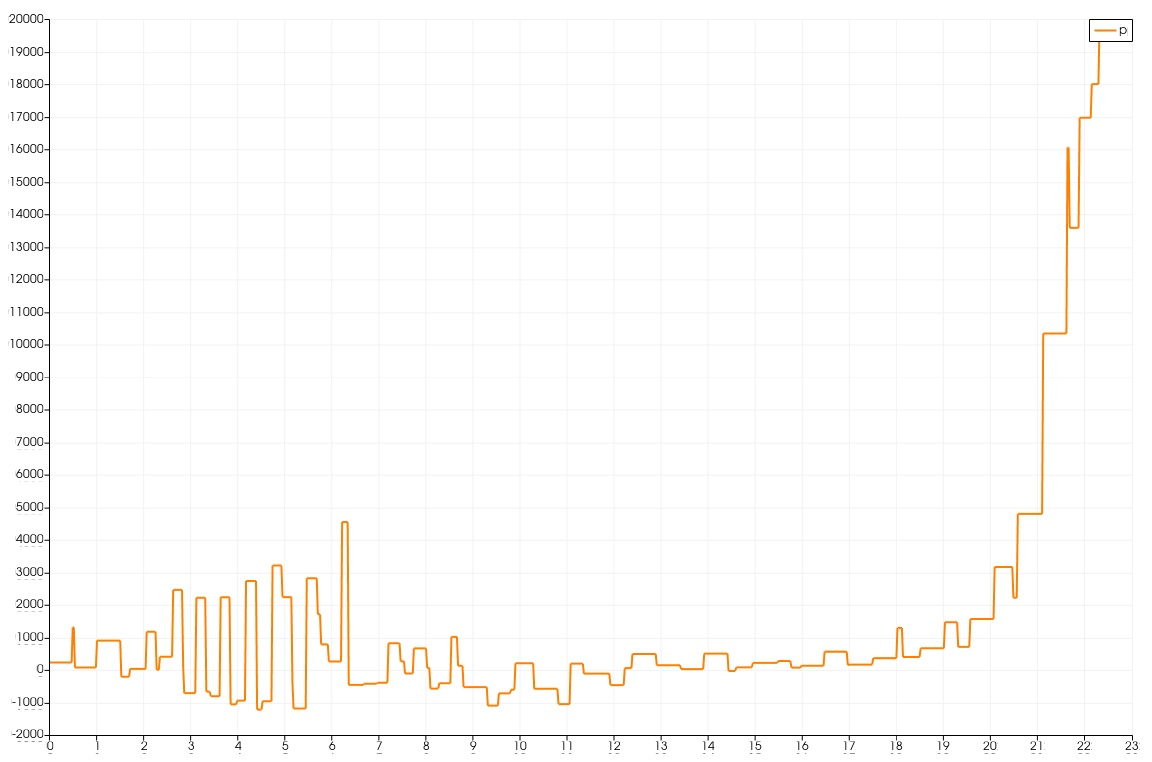
\includegraphics[width=\textwidth]{figures/ch9_q10_P_graphe.jpeg}
    \caption{Évolution de la pression $p$ (Pa) le long de l'axe longitudinal de l'évacuateur — débit décennal $Q_{10} = 160{,}74$ m³/s. La décroissance de pression le long du coursier et la surpression à la cuillère sont clairement identifiables.}
    \label{fig:q10_P_graphe}
\end{figure}

Le graphe de pression confirme les tendances observées sur le profil : la pression chute fortement à la crête du seuil (passage du régime fluvial au régime critique) puis continue de décroître sur le coursier torrentiel, avant d'augmenter légèrement à la cuillère sous l'effet de la courbure.

\subsection{Hauteur d'eau aux points caractéristiques}
\label{subsec:q10_hauteur}

Les figures suivantes présentent la hauteur d'eau aux trois points caractéristiques de l'ouvrage : le seuil, le coursier et la cuillère.

\begin{figure}[H]
    \centering
    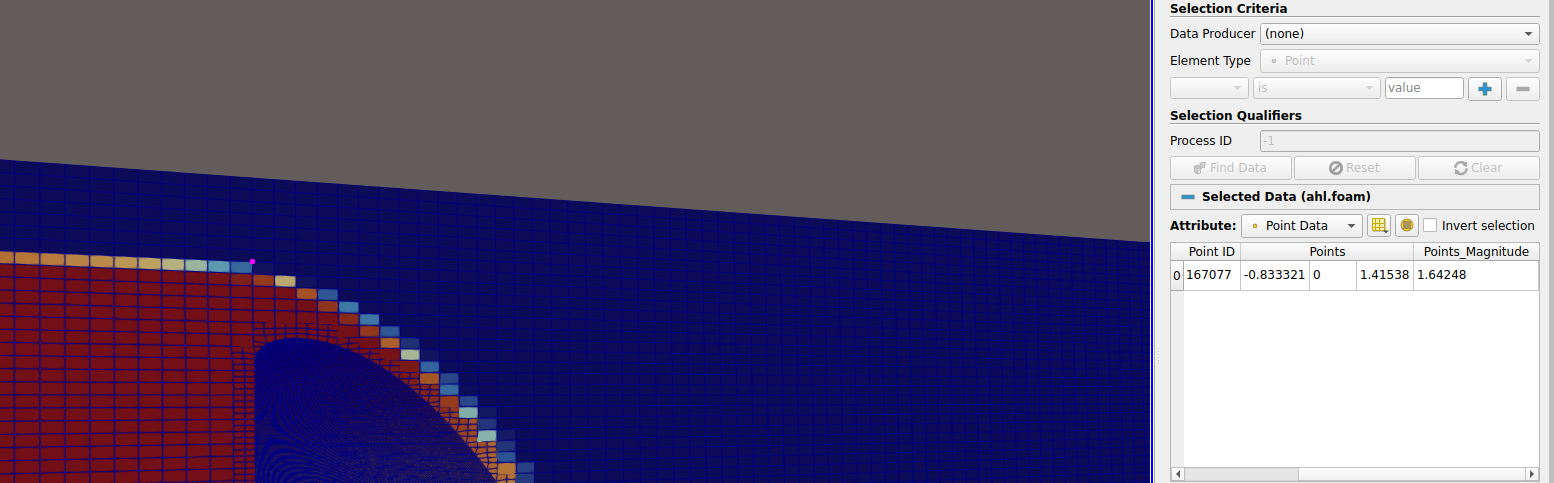
\includegraphics[width=\textwidth]{figures/ch9_q10_h_seuil.png}
    \caption{Hauteur d'eau au seuil Creager — débit décennal $Q_{10} = 160{,}74$ m³/s. La charge simulée sur le seuil est $H_d \approx 1{,}44$ m, lue sur le tableau de données ParaView (coordonnée verticale du point de surface libre sélectionné). Cette valeur correspond à la charge de déversement du seuil Creager (section \ref{sec:loi_debit_charge}).}
    \label{fig:q10_h_seuil}
\end{figure}

\begin{figure}[H]
    \centering
    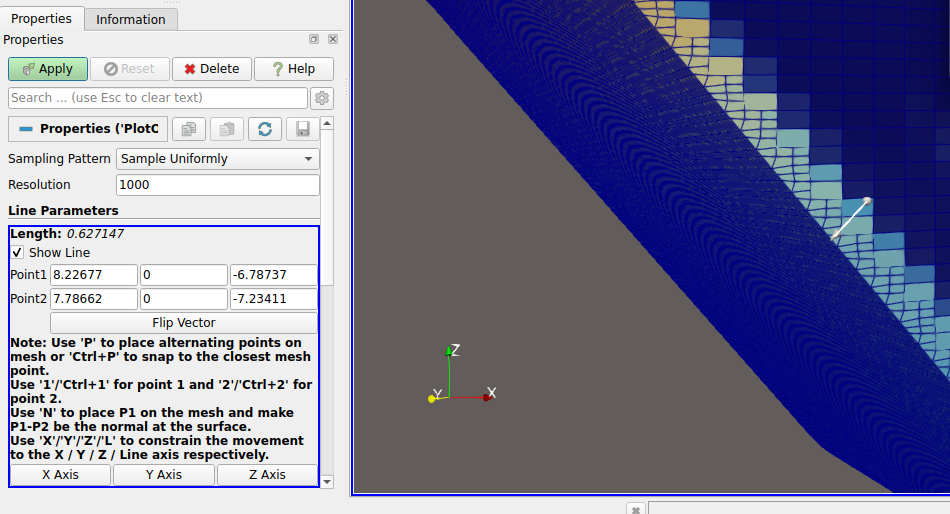
\includegraphics[width=\textwidth]{figures/ch9_q10_h_coursier.png}
    \caption{Hauteur d'eau sur le coursier — débit décennal $Q_{10} = 160{,}74$ m³/s. La hauteur de la lame d'eau mesurée par règle ParaView est $h_{\text{coursier}} = 0{,}40$ m. La lame d'eau s'amincit progressivement le long du coursier, traduisant l'accélération de l'écoulement supercritique.}
    \label{fig:q10_h_coursier}
\end{figure}

\begin{figure}[H]
    \centering
    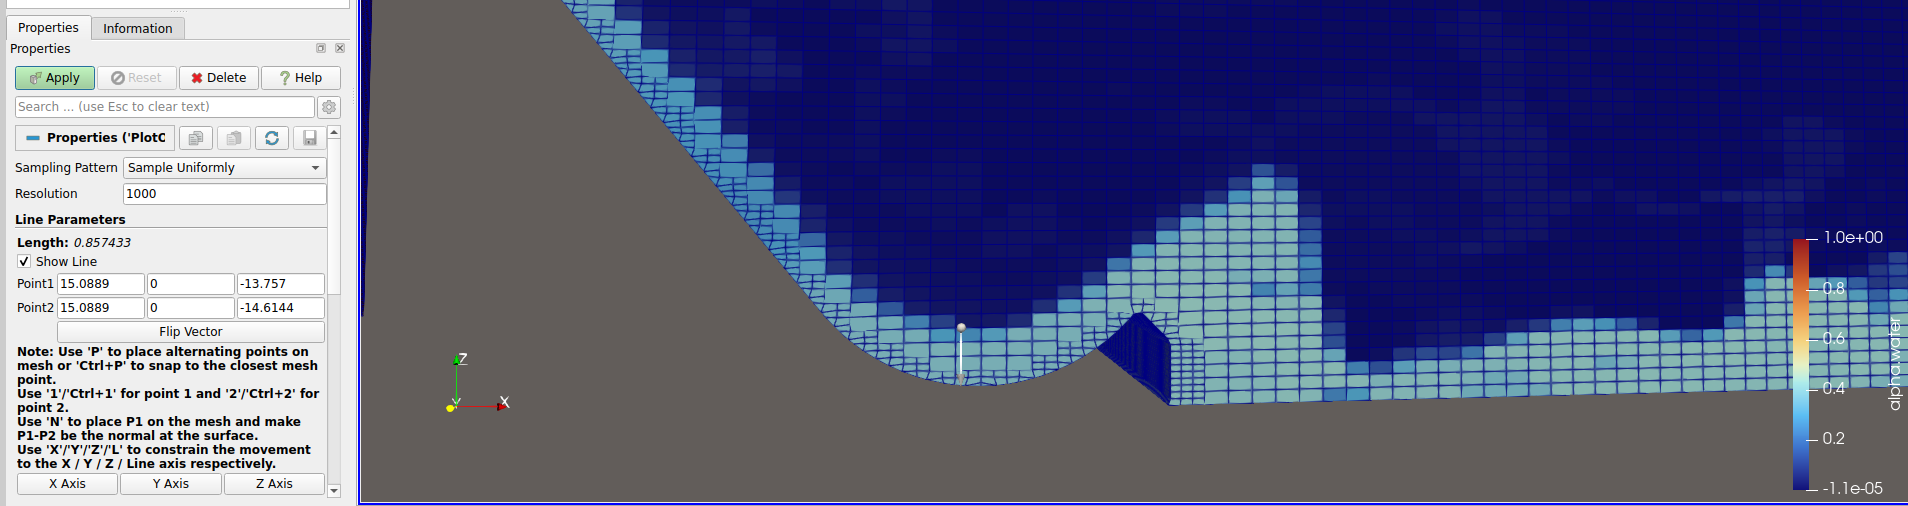
\includegraphics[width=\textwidth]{figures/ch9_q10_h_cuillere.png}
    \caption{Hauteur d'eau à la cuillère saut de ski — débit décennal $Q_{10} = 160{,}74$ m³/s. La hauteur est obtenue par la différence des coordonnées Z (tableau de gauche ParaView) : $z_1 = -13{,}757$ m et $z_2 = -14{,}614$ m, soit $h_{\text{cuillère}} = \Delta z = 0{,}857$ m. Cette hauteur est à comparer avec le dimensionnement de la cuillère (section \ref{sec:geometrie_cuillere}).}
    \label{fig:q10_h_cuillere}
\end{figure}

La progression des hauteurs d'eau confirme le comportement attendu : la lame est relativement épaisse au seuil (charge de déversement), s'amincit rapidement sur le coursier sous l'effet de l'accélération gravitationnelle, et atteint sa valeur minimale à la cuillère. Ces hauteurs sont cohérentes avec les résultats de la courbe de remous calculée sous HEC-RAS (annexe \ref{ann:hecras}).

\subsection{Jet et point d'impact}
\label{subsec:q10_jet}

\begin{figure}[H]
    \centering
    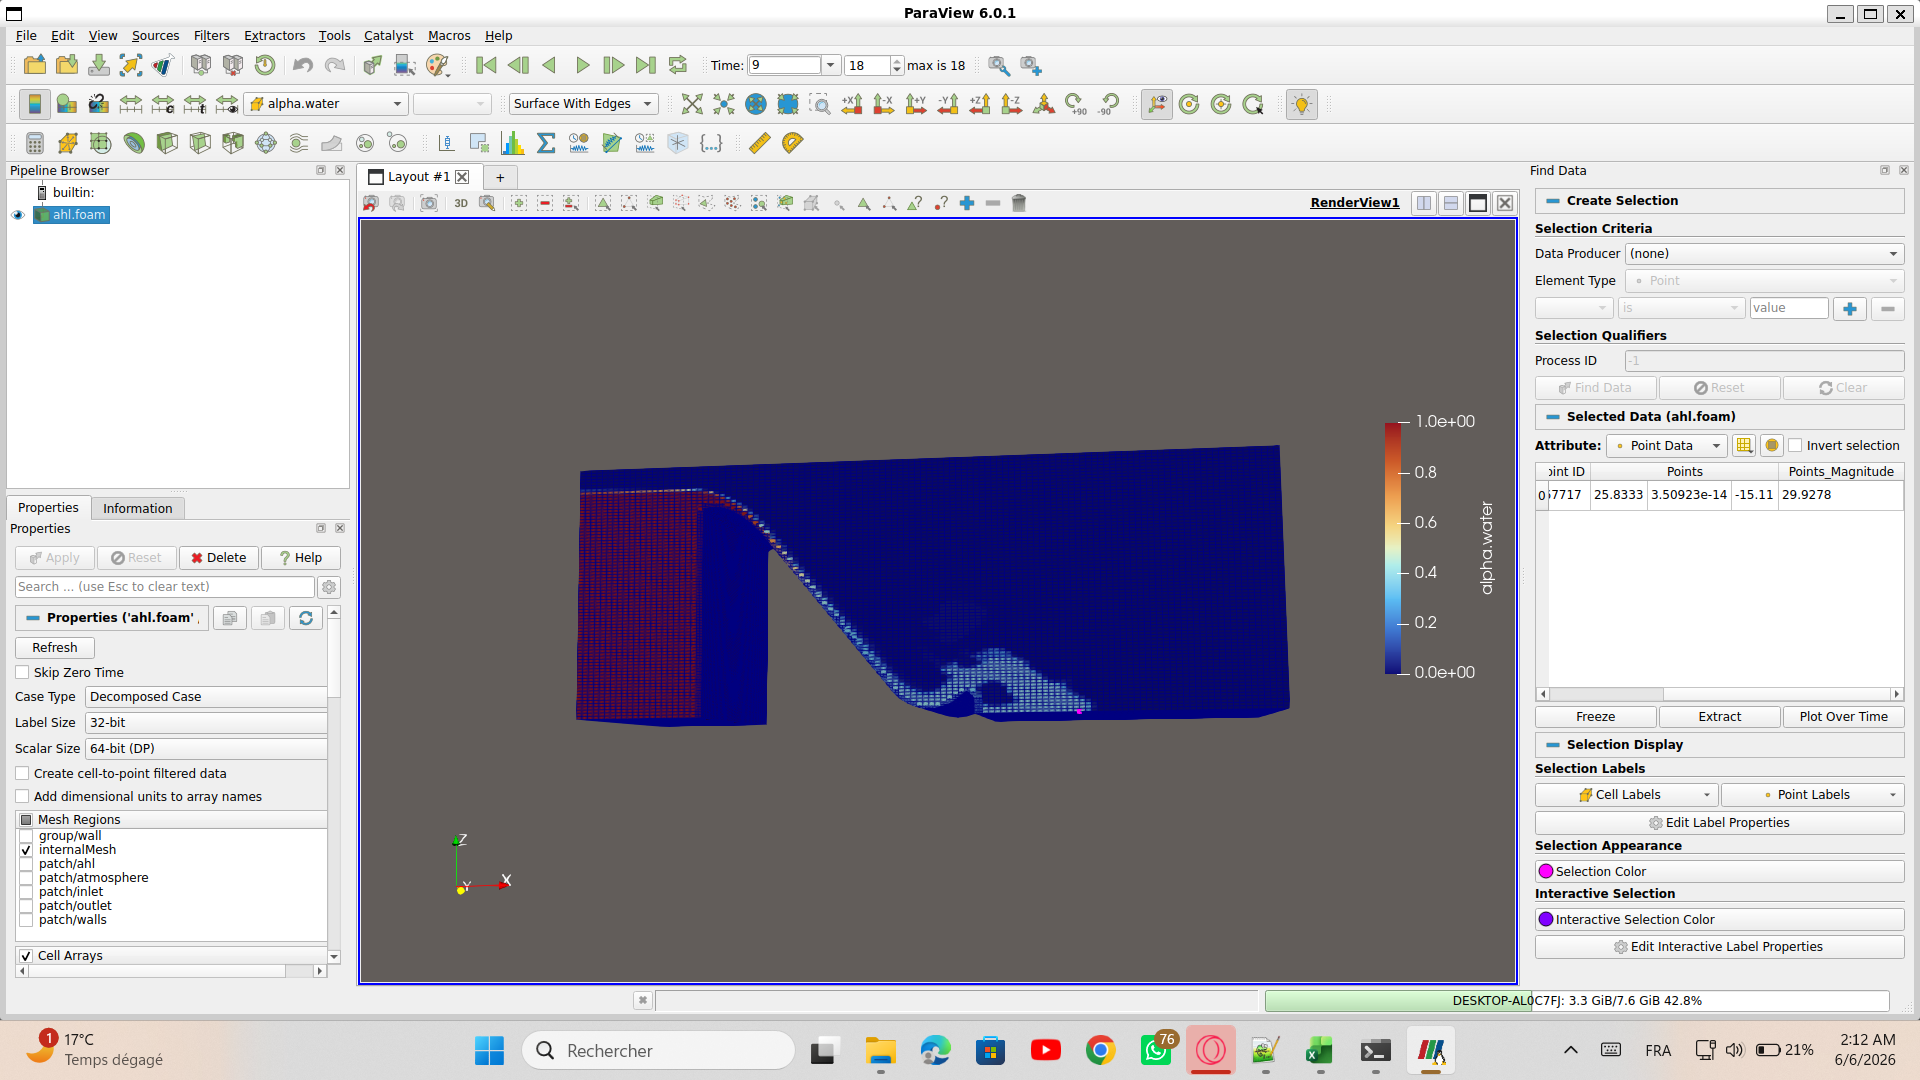
\includegraphics[width=\textwidth]{figures/ch9_q10_jet.png}
    \caption{Trajectoire du jet en aval de la cuillère saut de ski et point d'impact — débit décennal $Q_{10} = 160{,}74$ m³/s. Le point d'impact sélectionné a pour coordonnée $x = 25{,}83$ m ; le dernier point de la cuillère étant à $x = 16{,}72$ m, la distance de jet numérique est $L_x^{\text{num}} = 25{,}83 - 16{,}72 = \mathbf{9{,}11}$ \textbf{m}.}
    \label{fig:q10_jet}
\end{figure}

Pour le débit décennal, le jet issu de la cuillère suit une trajectoire parabolique cohérente avec la vitesse d'éjection et l'angle du bec déviateur. Le point d'impact, identifié dans ParaView à la coordonnée $x = 25{,}83$ m, donne une portée numérique $L_x^{\text{num}} = 25{,}83 - 16{,}72 = 9{,}11$ m mesurée à l'intérieur du domaine de calcul. La localisation du point d'impact détermine la zone d'affouillement potentielle et conditionne les mesures de protection du lit aval (section \ref{sec:affouillement}).

% ============================================================
%  SECTION 9.2 : Q100
% ============================================================
\section{Résultats pour le débit centennal $Q_{100} = 507{,}54$ m³/s}
\label{sec:resultats_q100}

\subsection{Champ de vitesse}
\label{subsec:q100_vitesse}

\begin{figure}[H]
    \centering
    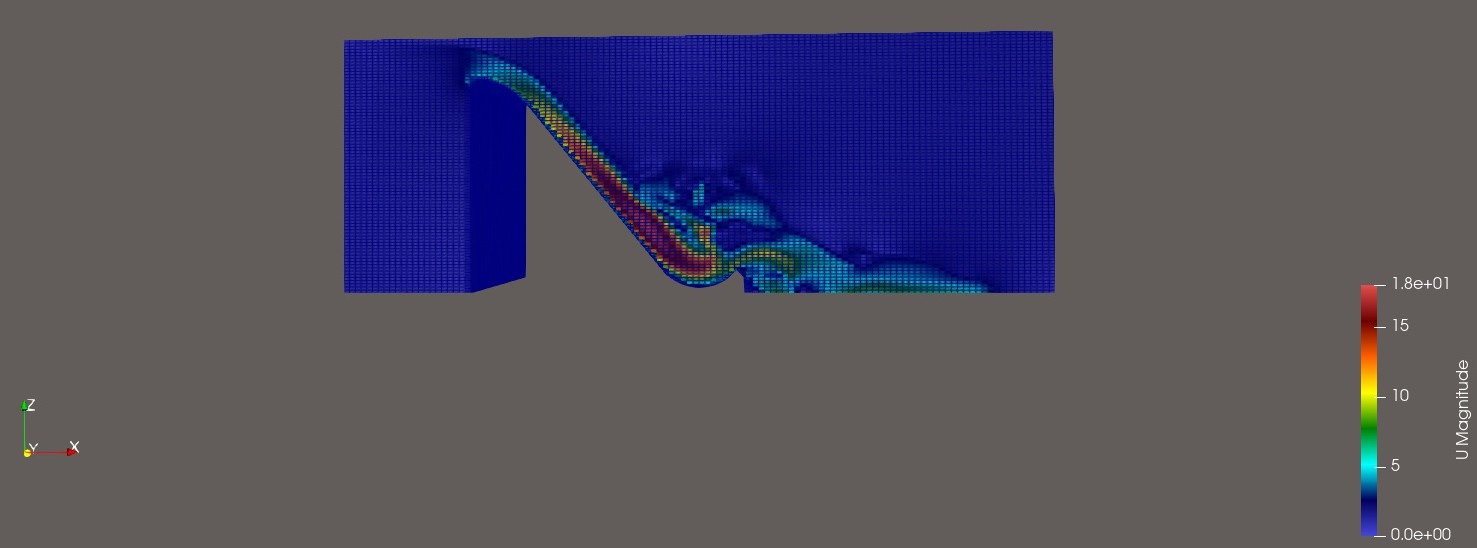
\includegraphics[width=\textwidth]{figures/ch9_q100_U_profil.jpeg}
    \caption{Profil du champ de vitesse $\|\mathbf{U}\|$ (m/s) le long de l'évacuateur de crues — débit centennal $Q_{100} = 507{,}54$ m³/s. Par rapport au débit décennal, les vitesses sont notablement plus élevées sur l'ensemble du coursier.}
    \label{fig:q100_U_profil}
\end{figure}

\begin{figure}[H]
    \centering
    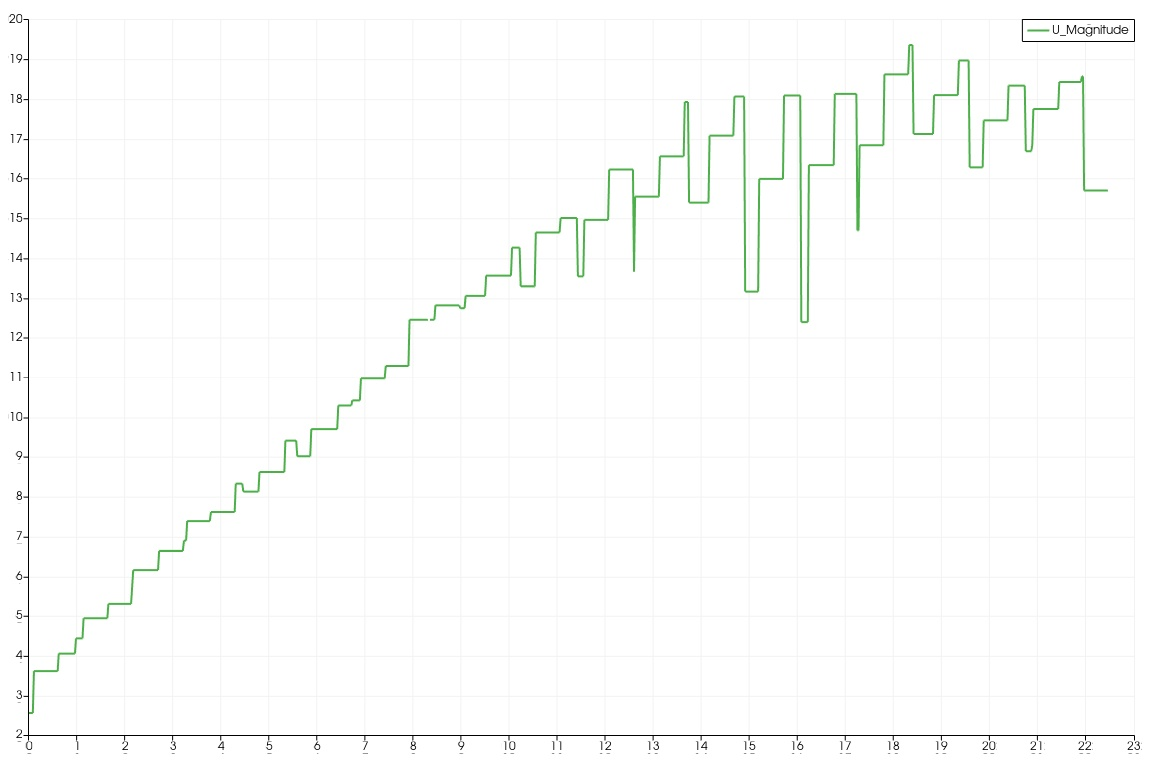
\includegraphics[width=\textwidth]{figures/ch9_q100_U_graphe.jpeg}
    \caption{Évolution de la vitesse $\|\mathbf{U}\|$ (m/s) le long de l'axe longitudinal de l'évacuateur — débit centennal $Q_{100} = 507{,}54$ m³/s.}
    \label{fig:q100_U_graphe}
\end{figure}

Pour le débit centennal, les vitesses sont significativement plus élevées que pour $Q_{10}$, reflet de l'augmentation du débit spécifique. L'accélération reste progressive le long du coursier, mais les valeurs maximales à la cuillère sont plus importantes, ce qui se traduit par une énergie cinétique plus grande et une portée de jet accrue.

\subsection{Champ de pression}
\label{subsec:q100_pression}

\begin{figure}[H]
    \centering
    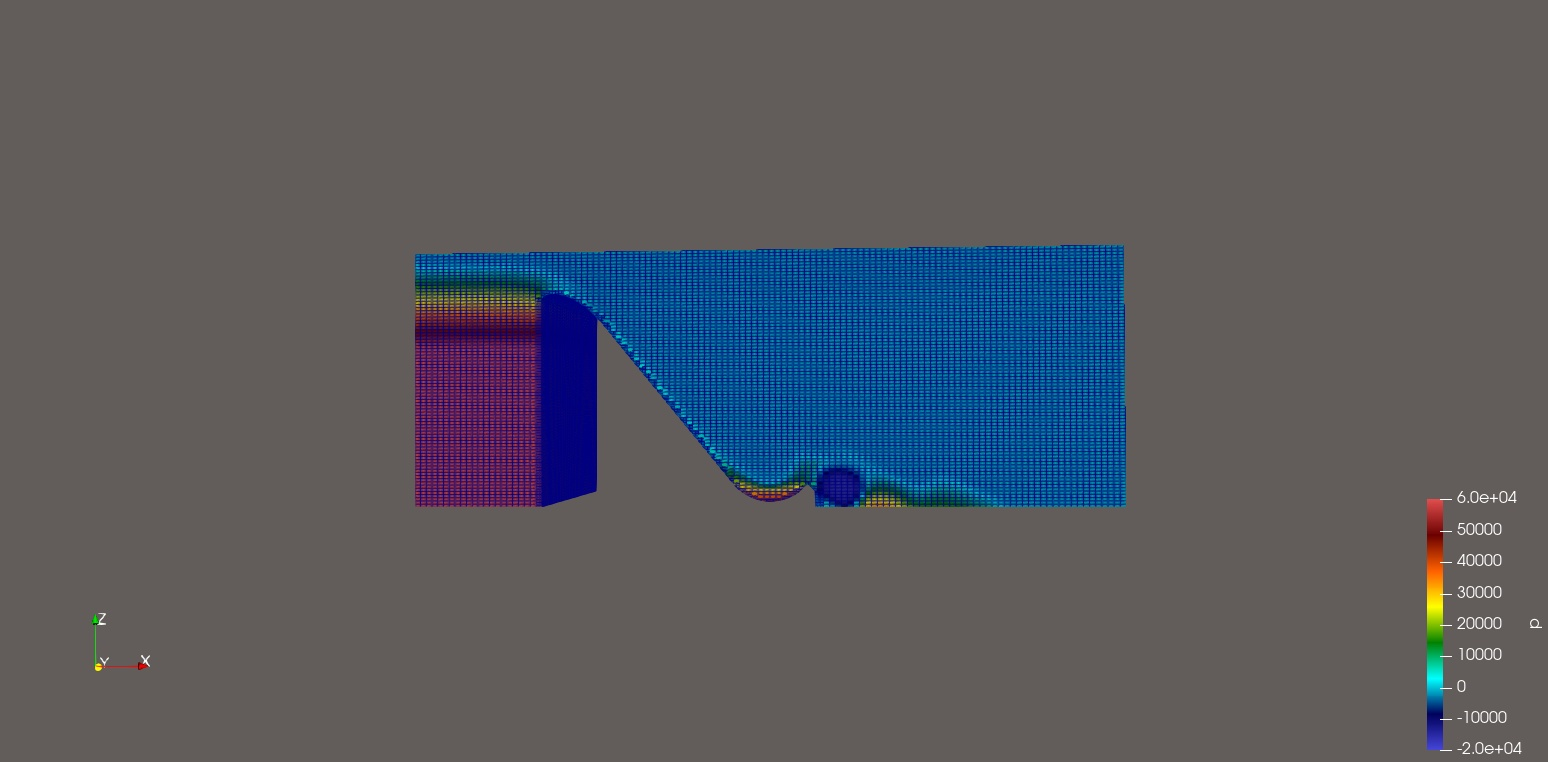
\includegraphics[width=\textwidth]{figures/ch9_q100_P_profil.jpeg}
    \caption{Profil du champ de pression $p$ (Pa) le long de l'évacuateur de crues — débit centennal $Q_{100} = 507{,}54$ m³/s. La surpression à la cuillère est plus prononcée qu'à $Q_{10}$, en raison des vitesses plus élevées.}
    \label{fig:q100_P_profil}
\end{figure}

\begin{figure}[H]
    \centering
    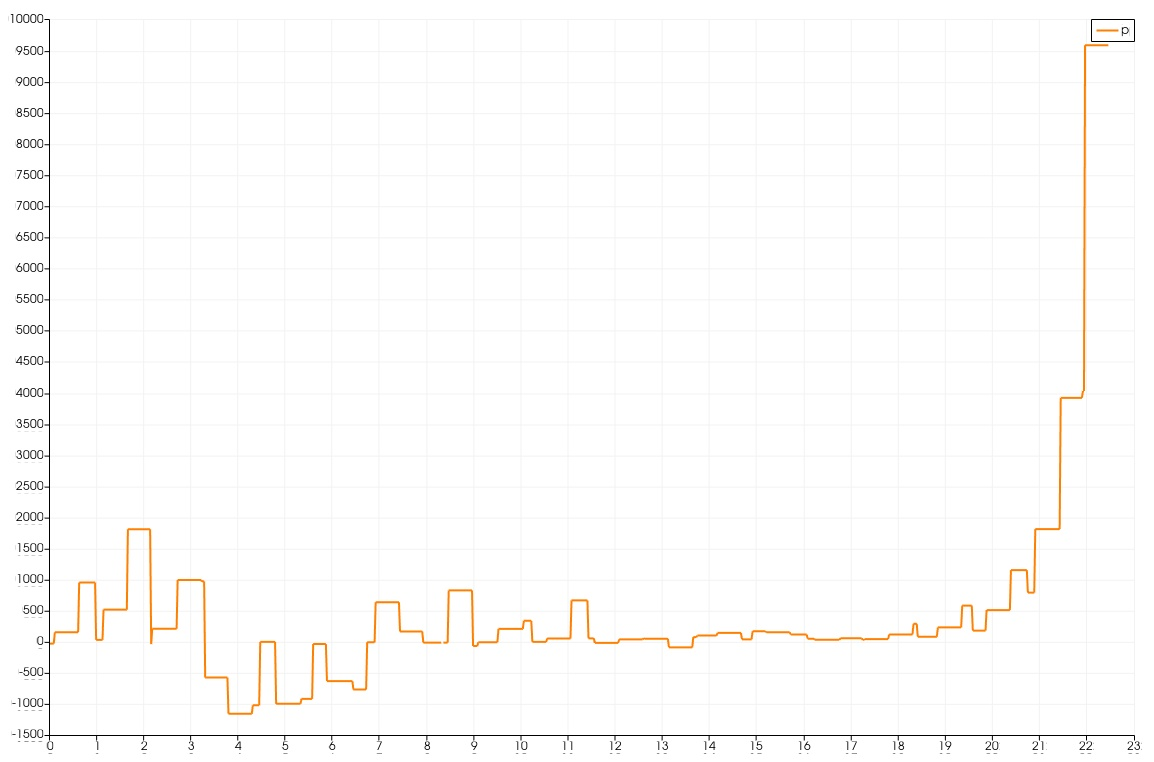
\includegraphics[width=\textwidth]{figures/ch9_q100_P_graphe.jpeg}
    \caption{Évolution de la pression $p$ (Pa) le long de l'axe longitudinal de l'évacuateur — débit centennal $Q_{100} = 507{,}54$ m³/s.}
    \label{fig:q100_P_graphe}
\end{figure}

La distribution de pression pour $Q_{100}$ présente les mêmes tendances générales que pour $Q_{10}$, avec une intensification des pressions dans la retenue (charge plus élevée) et une surpression plus marquée à la cuillère, liée à l'augmentation des forces centrifuges avec la vitesse. Ces valeurs restent compatibles avec les contraintes structurelles de l'ouvrage.

\subsection{Hauteur d'eau aux points caractéristiques}
\label{subsec:q100_hauteur}

\begin{figure}[H]
    \centering
    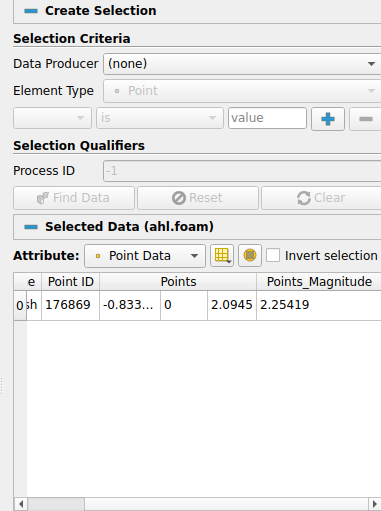
\includegraphics[width=0.75\textwidth]{figures/ch9_q100_h_seuil.png}
    \caption{Hauteur d'eau au seuil Creager — débit centennal $Q_{100} = 507{,}54$ m³/s. La charge simulée est $H_d \approx 2{,}09$ m, lue directement sur la coordonnée verticale du point de surface libre sélectionné dans le tableau de données ParaView. La charge sur le seuil est plus importante qu'à $Q_{10}$, conformément à la loi débit-charge (section \ref{sec:loi_debit_charge}).}
    \label{fig:q100_h_seuil}
\end{figure}

\begin{figure}[H]
    \centering
    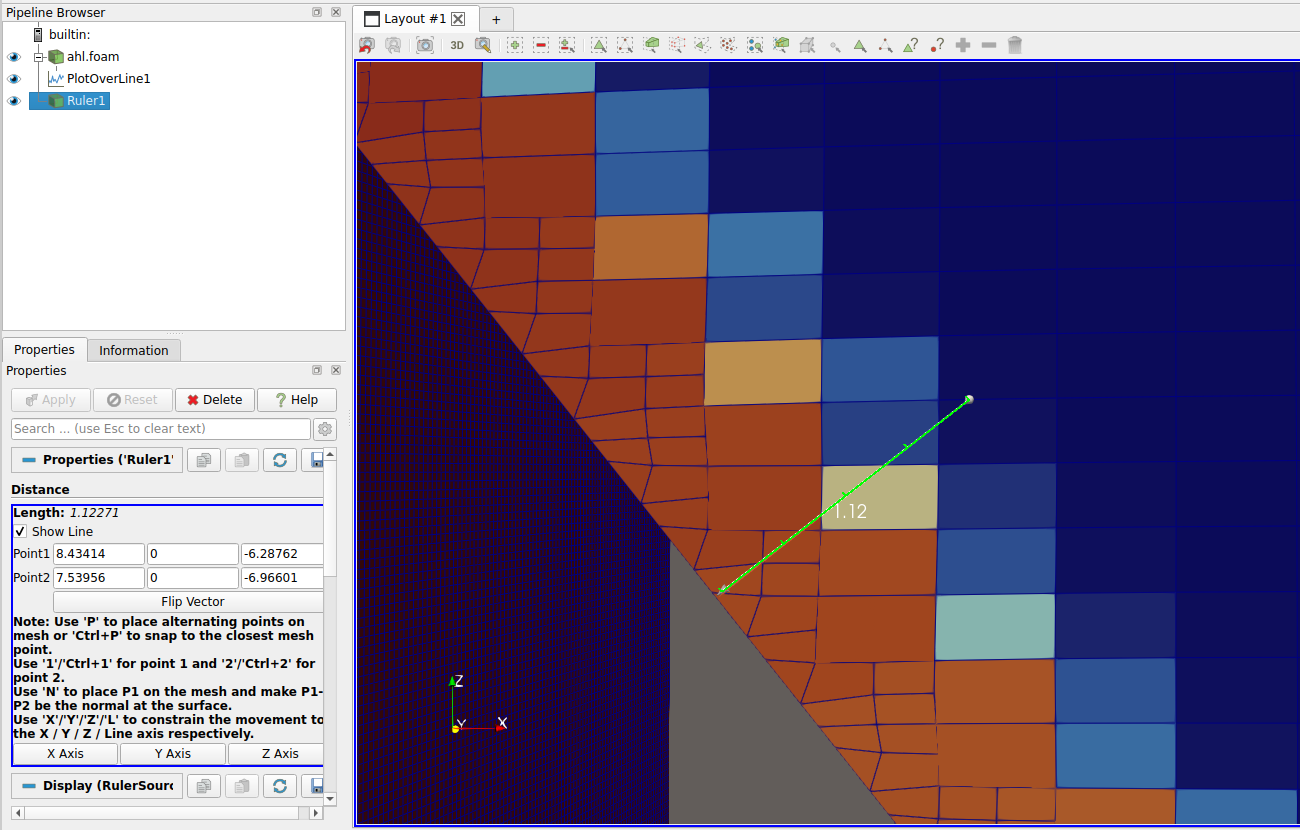
\includegraphics[width=\textwidth]{figures/ch9_q100_h_coursier.png}
    \caption{Hauteur d'eau sur le coursier — débit centennal $Q_{100} = 507{,}54$ m³/s. La hauteur de la lame d'eau est lue directement sur la flèche de la règle ParaView : $h_{\text{coursier}} = 1{,}12$ m. Cette valeur, supérieure à celle obtenue pour $Q_{10}$, implique une hauteur de murs bajoyers plus importante.}
    \label{fig:q100_h_coursier}
\end{figure}

\begin{figure}[H]
    \centering
    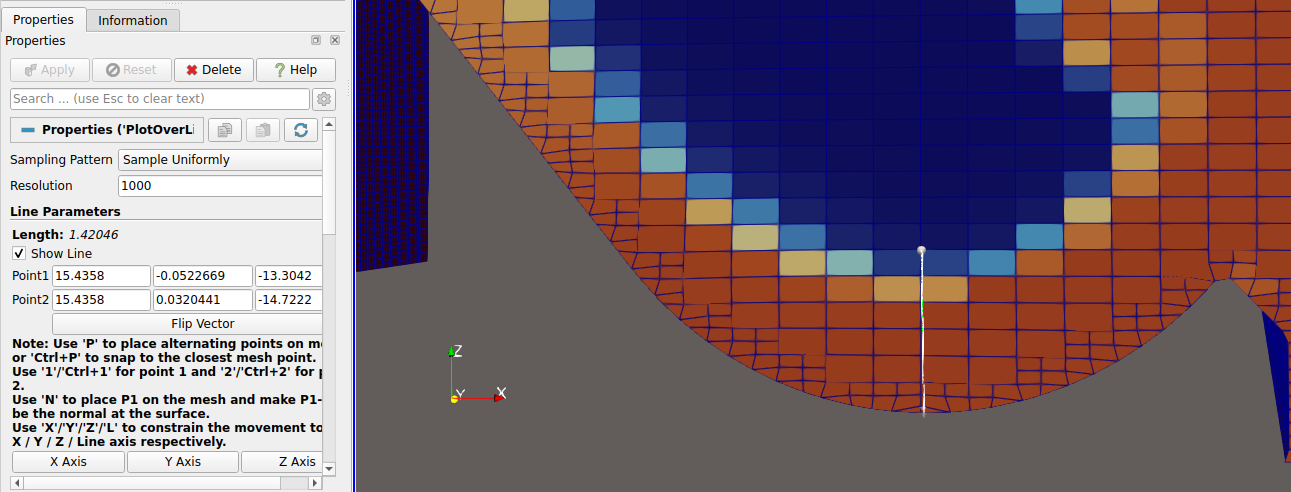
\includegraphics[width=\textwidth]{figures/ch9_q100_h_cuillere.png}
    \caption{Hauteur d'eau à la cuillère saut de ski — débit centennal $Q_{100} = 507{,}54$ m³/s. La hauteur est obtenue par la différence des coordonnées Z (tableau de gauche ParaView) : $z_1 = -13{,}30$ m et $z_2 = -14{,}72$ m, soit $h_{\text{cuillère}} = \Delta z = 1{,}42$ m.}
    \label{fig:q100_h_cuillere}
\end{figure}

La comparaison des hauteurs d'eau entre $Q_{10}$ et $Q_{100}$ met en évidence l'augmentation de la lame d'eau sur l'ensemble de l'ouvrage. La hauteur sur le coursier, plus importante pour $Q_{100}$, conforte le dimensionnement des murs bajoyers réalisé à la section \ref{sec:murs_bajoyers}.

\subsection{Jet et point d'impact}
\label{subsec:q100_jet}

\begin{figure}[H]
    \centering
    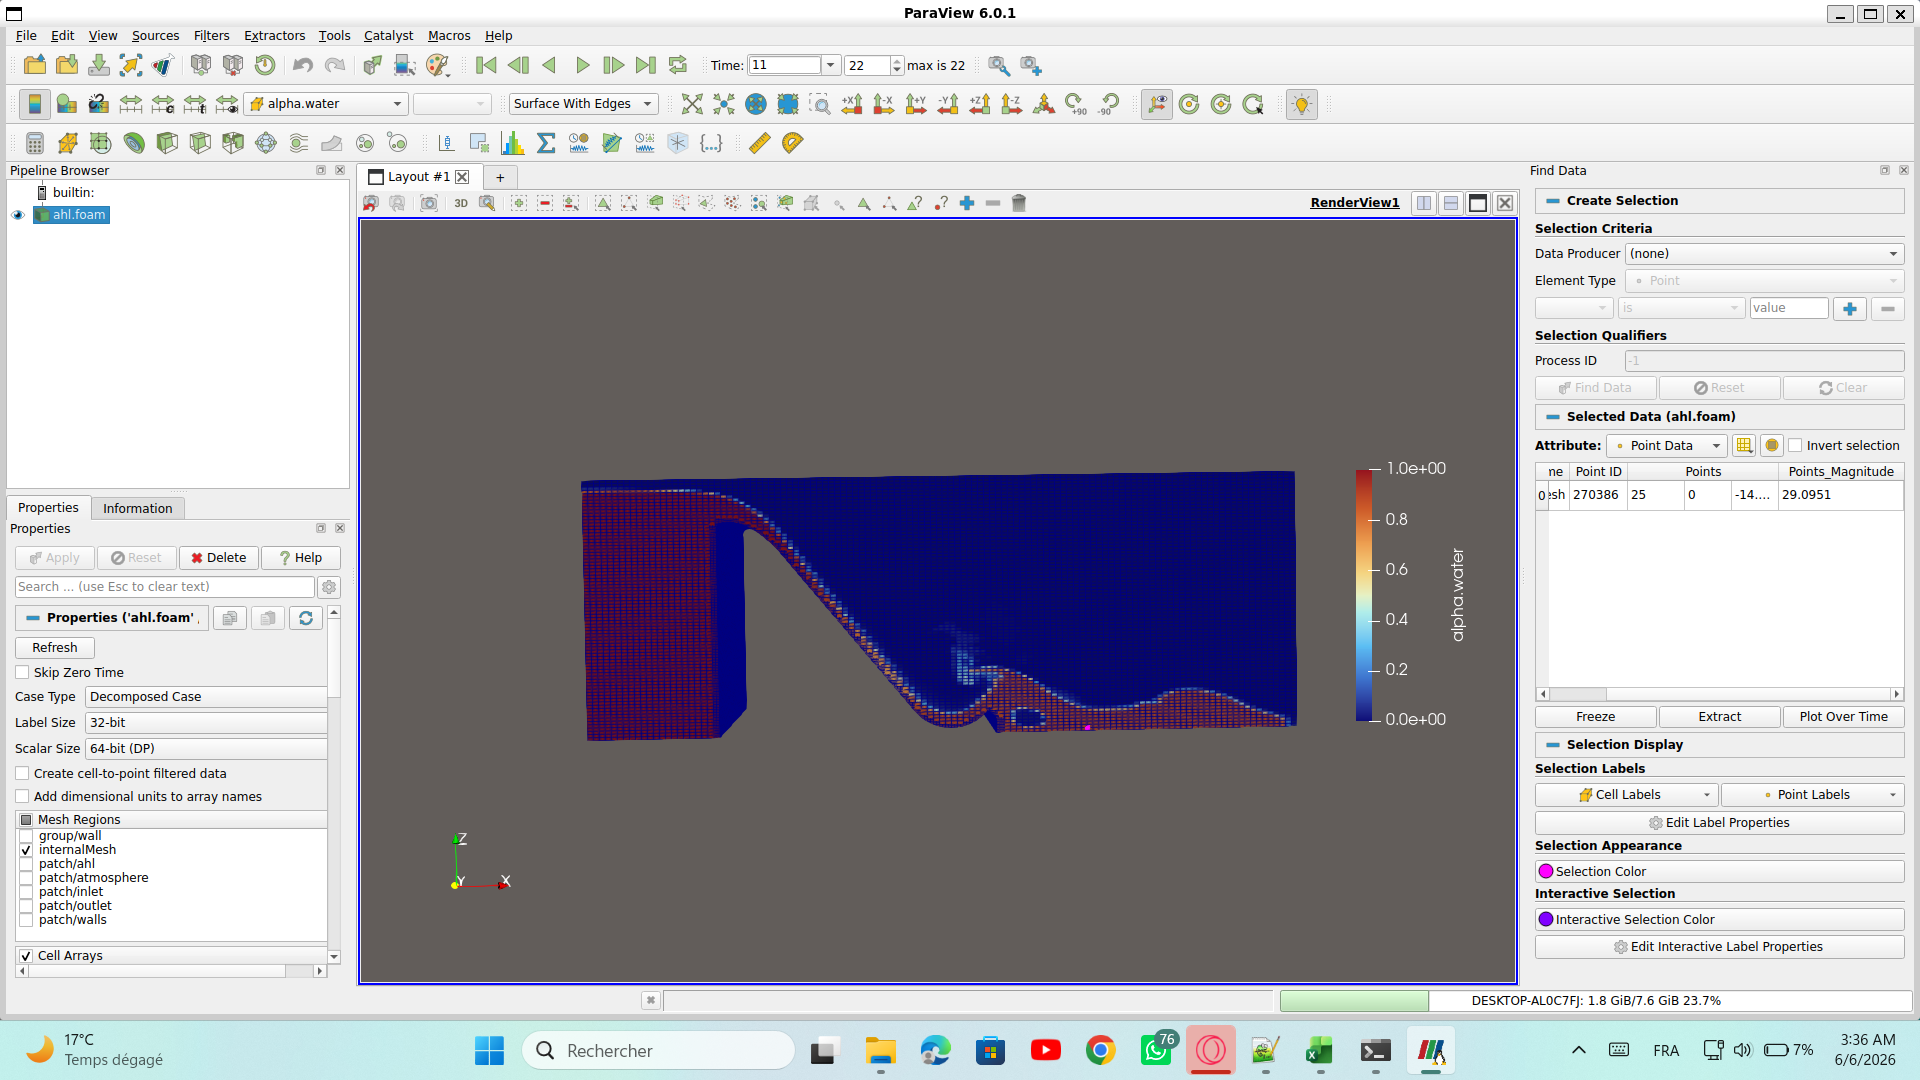
\includegraphics[width=\textwidth]{figures/ch9_q100_jet.png}
    \caption{Trajectoire du jet en aval de la cuillère saut de ski et point d'impact — débit centennal $Q_{100} = 507{,}54$ m³/s. Le point d'impact sélectionné a pour coordonnée $x \approx 25{,}0$ m ; la distance de jet numérique est $L_x^{\text{num}} = 25{,}0 - 16{,}72 = \mathbf{8{,}28}$ \textbf{m}.}
    \label{fig:q100_jet}
\end{figure}

Pour $Q_{100}$, la trajectoire du jet est légèrement différente de celle de $Q_{10}$ en raison de la vitesse d'éjection plus élevée. Le point d'impact identifié dans ParaView a pour coordonnée $x \approx 25{,}0$ m, donnant une portée numérique $L_x^{\text{num}} = 25{,}0 - 16{,}72 = 8{,}28$ m. Le point d'impact détermine la zone de protection à prévoir sur le lit de l'oued en aval de l'ouvrage.

% ============================================================
%  SECTION 9.3 : Q1000
% ============================================================
\section{Résultats pour le débit millénal $Q_{1\,000} = 794{,}93$ m³/s}
\label{sec:resultats_q1000}

\subsection{Champ de vitesse}
\label{subsec:q1000_vitesse}

\begin{figure}[H]
    \centering
    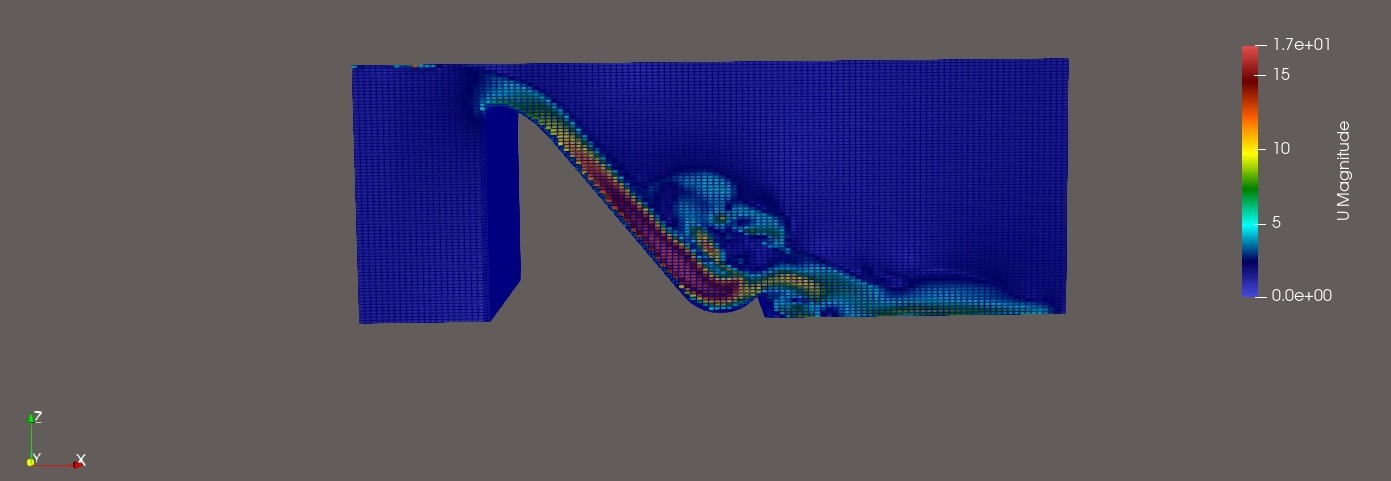
\includegraphics[width=\textwidth]{figures/ch9_q1000_U_profil.jpeg}
    \caption{Profil du champ de vitesse $\|\mathbf{U}\|$ (m/s) le long de l'évacuateur de crues — débit millénal $Q_{1\,000} = 794{,}93$ m³/s. Ce cas constitue le scénario le plus sollicitant : les vitesses sur le coursier et à la cuillère atteignent leurs valeurs maximales parmi les trois débits étudiés.}
    \label{fig:q1000_U_profil}
\end{figure}

\begin{figure}[H]
    \centering
    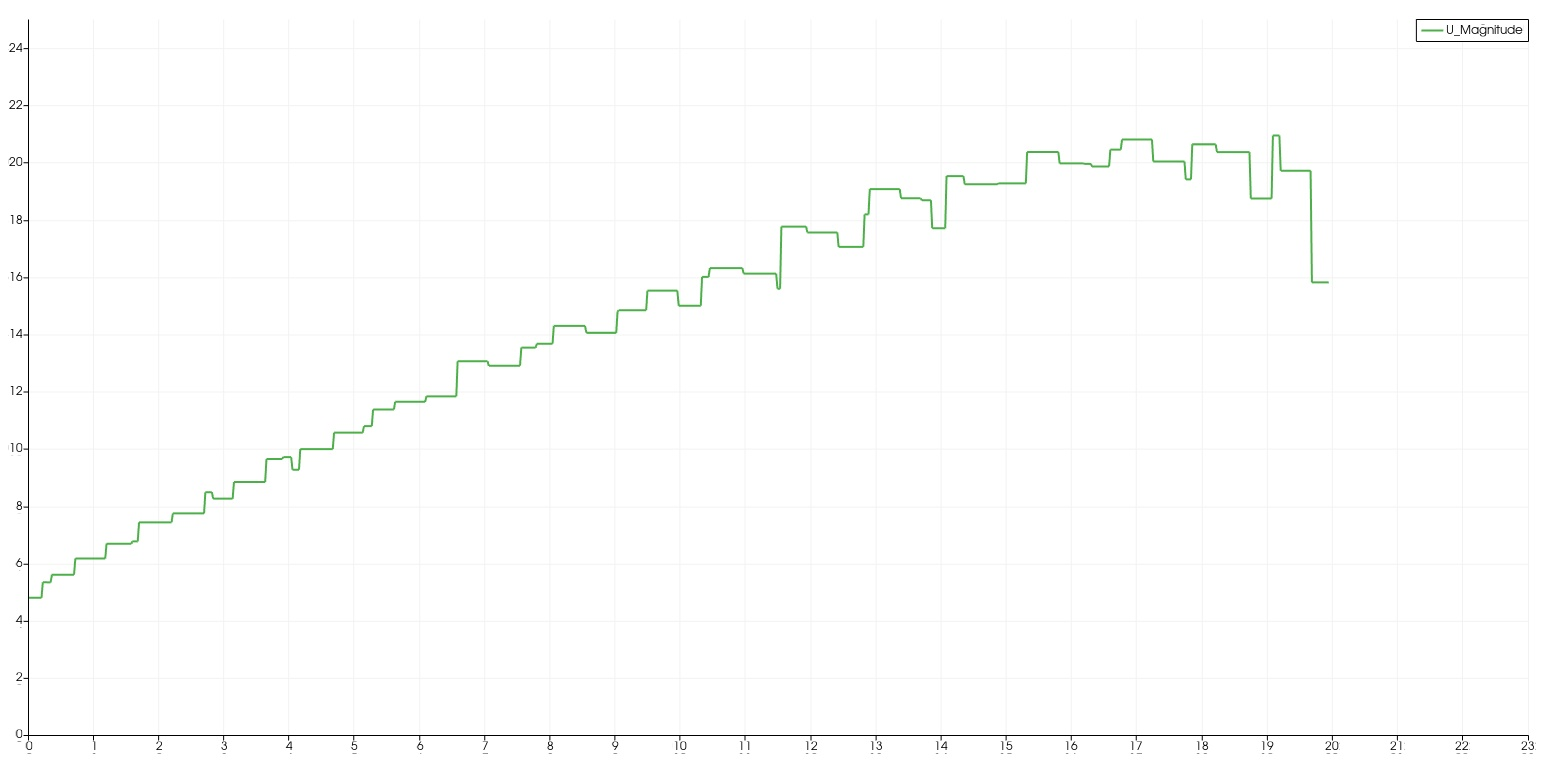
\includegraphics[width=\textwidth]{figures/ch9_q1000_U_graphe.jpeg}
    \caption{Évolution de la vitesse $\|\mathbf{U}\|$ (m/s) le long de l'axe longitudinal de l'évacuateur — débit millénal $Q_{1\,000} = 794{,}93$ m³/s.}
    \label{fig:q1000_U_graphe}
\end{figure}

Le débit millénal constitue le cas le plus défavorable de l'étude. Les vitesses atteintes sur le coursier et à la cuillère sont les plus élevées des trois scénarios. Cette configuration est également celle pour laquelle le risque d'aération de la lame (entraînement d'air en surface) est le plus important, phénomène visible sur le profil de vitesse par les gradients plus diffus de l'interface eau/air.

\subsection{Champ de pression}
\label{subsec:q1000_pression}

\begin{figure}[H]
    \centering
    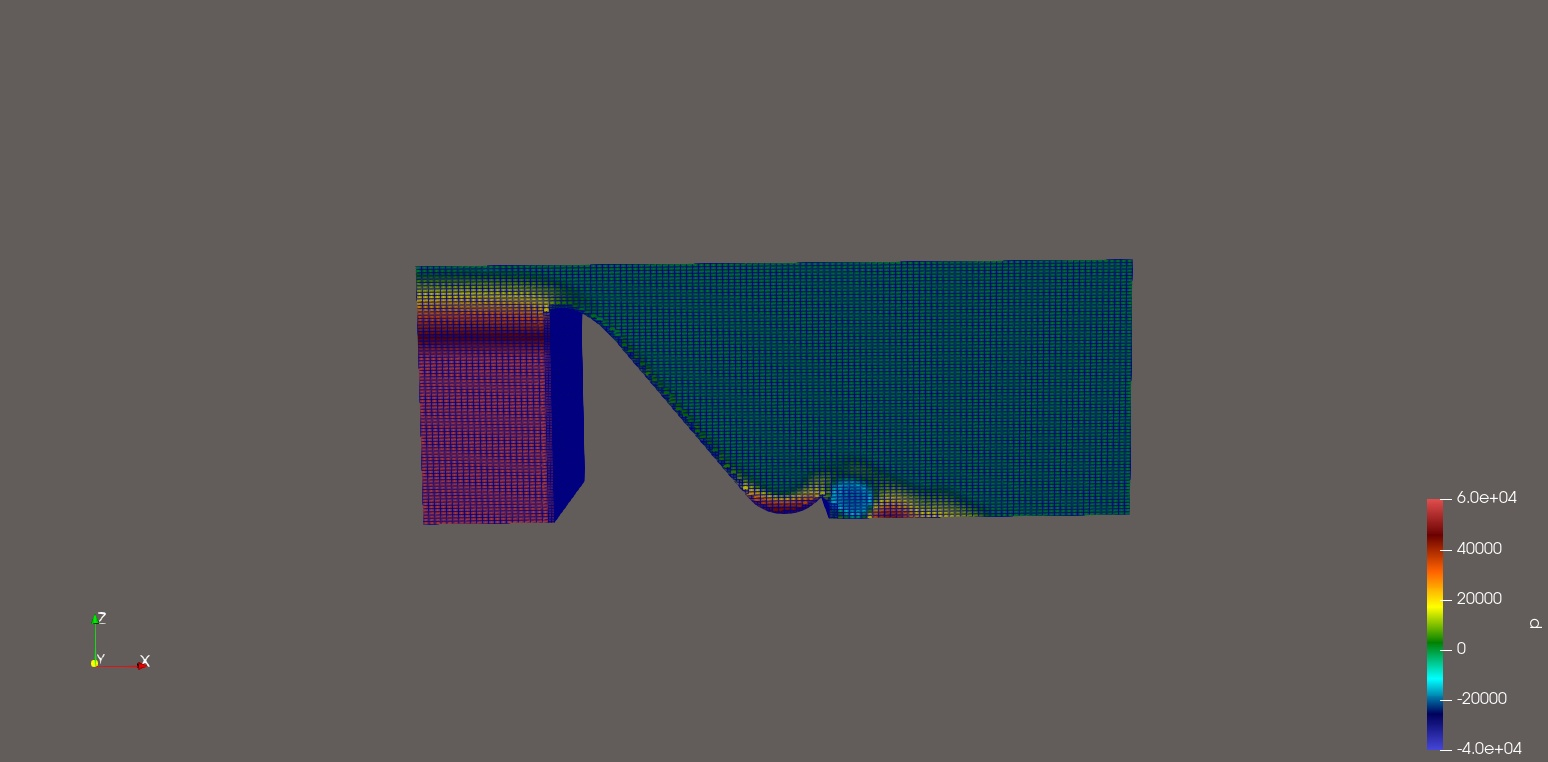
\includegraphics[width=\textwidth]{figures/ch9_q1000_P_profil.jpeg}
    \caption{Profil du champ de pression $p$ (Pa) le long de l'évacuateur de crues — débit millénal $Q_{1\,000} = 794{,}93$ m³/s. La surpression à la cuillère est maximale pour ce débit et constitue un paramètre de vérification structurelle de l'ouvrage.}
    \label{fig:q1000_P_profil}
\end{figure}

\begin{figure}[H]
    \centering
    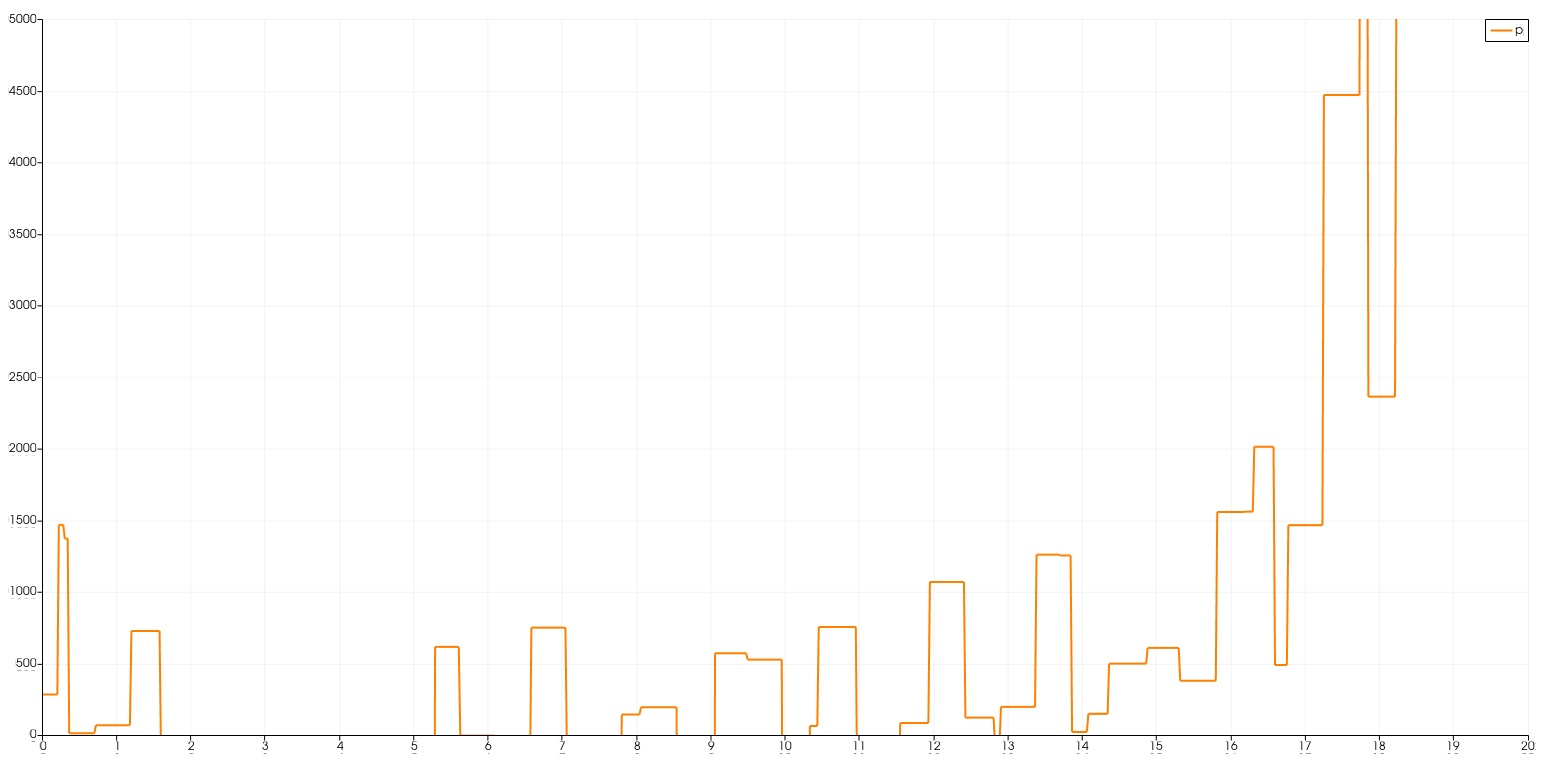
\includegraphics[width=\textwidth]{figures/ch9_q1000_P_graphe.jpeg}
    \caption{Évolution de la pression $p$ (Pa) le long de l'axe longitudinal de l'évacuateur — débit millénal $Q_{1\,000} = 794{,}93$ m³/s.}
    \label{fig:q1000_P_graphe}
\end{figure}

Pour $Q_{1\,000}$, la surpression à la cuillère atteint son niveau maximal parmi les trois débits simulés. Cette surpression, liée aux forces centrifuges exercées par la déviation du jet sur la surface courbe de la cuillère, est à vérifier vis-à-vis des contraintes admissibles du béton de l'ouvrage. La distribution de pression le long du coursier reste conforme à la théorie pour un écoulement supercritique : décroissance continue avec l'accélération, sans décollement ou dépression susceptible de provoquer de la cavitation sur les sections droites.

\subsection{Hauteur d'eau aux points caractéristiques}
\label{subsec:q1000_hauteur}

\begin{figure}[H]
    \centering
    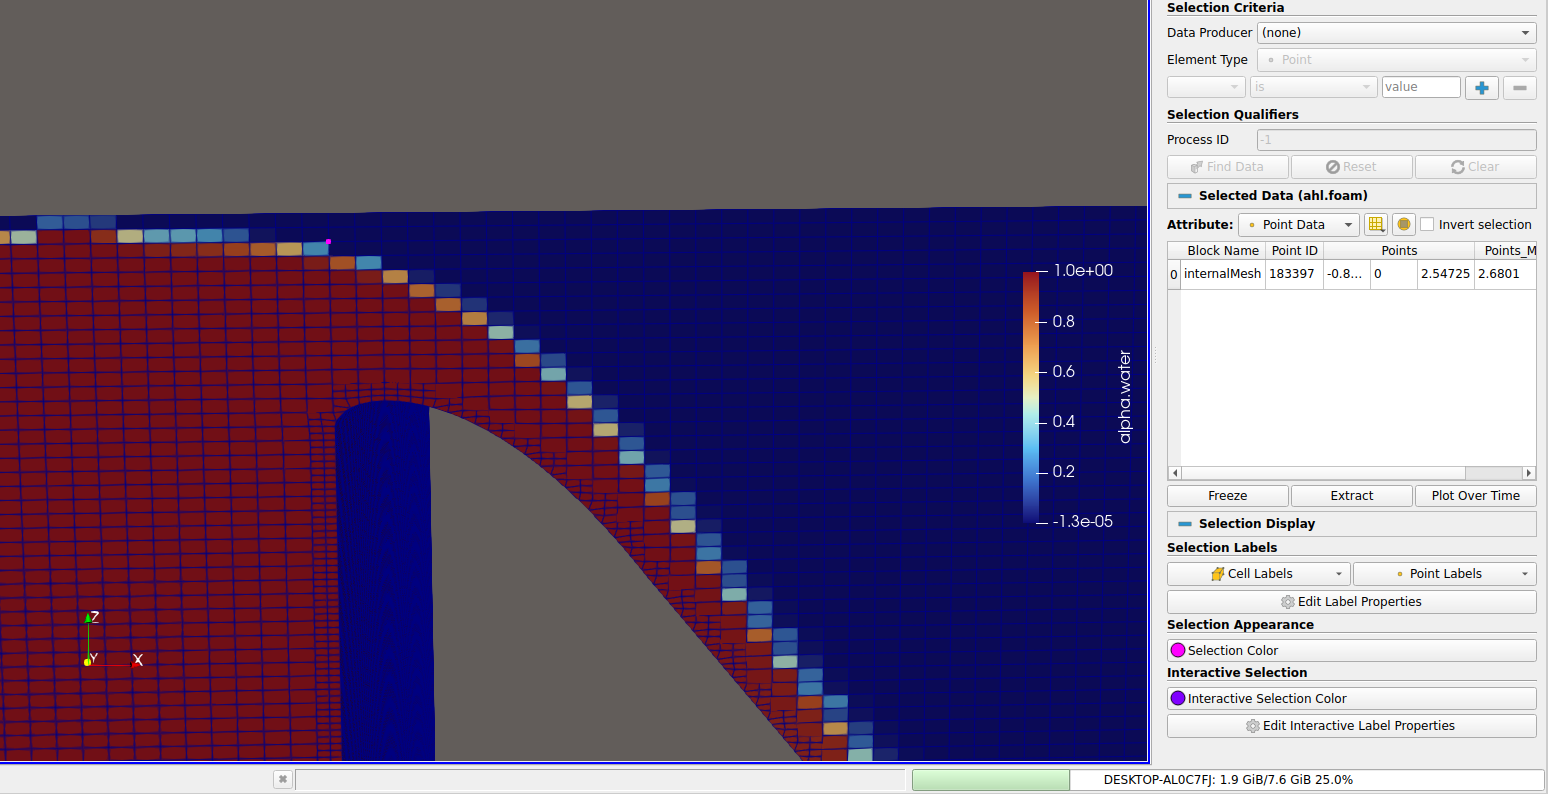
\includegraphics[width=\textwidth]{figures/ch9_q1000_h_seuil.png}
    \caption{Hauteur d'eau au seuil Creager — débit millénal $Q_{1\,000} = 794{,}93$ m³/s. La charge simulée est $H_d \approx 2{,}36$ m, valeur maximale parmi les trois débits étudiés, lue sur le tableau de données ParaView. Elle correspond à la charge de vérification de l'ouvrage.}
    \label{fig:q1000_h_seuil}
\end{figure}

\begin{figure}[H]
    \centering
    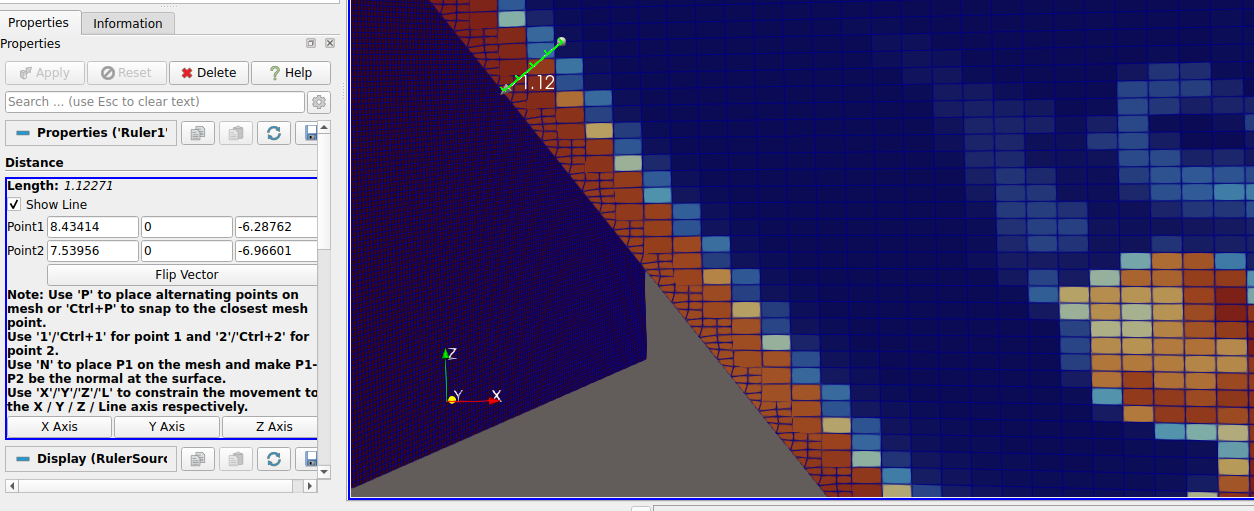
\includegraphics[width=\textwidth]{figures/ch9_q1000_h_coursier.png}
    \caption{Hauteur d'eau sur le coursier — débit millénal $Q_{1\,000} = 794{,}93$ m³/s. La hauteur mesurée par règle ParaView est $h_{\text{coursier}} \approx 0{,}82$ m, valeur la plus importante des trois débits simulés. Cette hauteur justifie le dimensionnement des murs bajoyers à la section \ref{sec:murs_bajoyers}.}
    \label{fig:q1000_h_coursier}
\end{figure}

\begin{figure}[H]
    \centering
    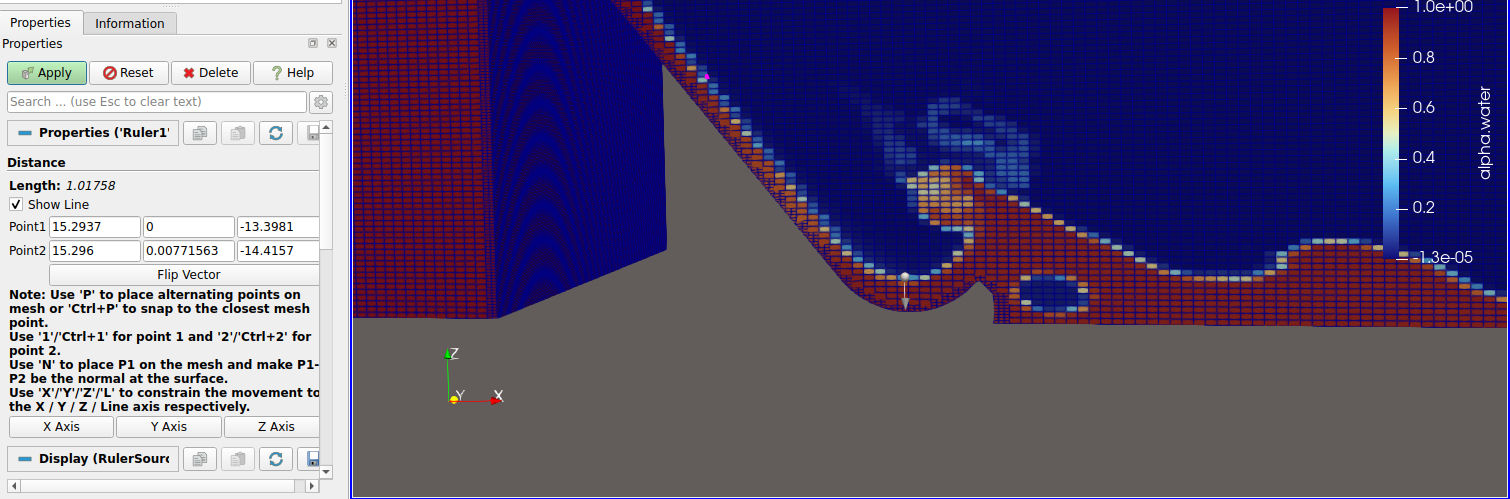
\includegraphics[width=\textwidth]{figures/ch9_q1000_h_cuillere.png}
    \caption{Hauteur d'eau à la cuillère saut de ski — débit millénal $Q_{1\,000} = 794{,}93$ m³/s. La hauteur mesurée dans ParaView est $h_{\text{cuillère}} = 0{,}61$ m.}
    \label{fig:q1000_h_cuillere}
\end{figure}

Pour le débit millénal, la hauteur d'eau sur le coursier est de $1{,}12$ m et à la cuillère de $1{,}01$ m. La hauteur sur le coursier constitue la valeur de référence pour le dimensionnement des murs bajoyers : elle confirme que la hauteur retenue au chapitre \ref{chap:dimensionnement_theorique} est suffisante pour contenir l'écoulement dans les conditions les plus défavorables. La faible hauteur d'eau à la cuillère ($1{,}01$ m), associée à une vitesse très élevée, traduit bien le caractère torrentiel extrême de l'écoulement à ce stade.

\subsection{Jet et point d'impact}
\label{subsec:q1000_jet}

\begin{figure}[H]
    \centering
    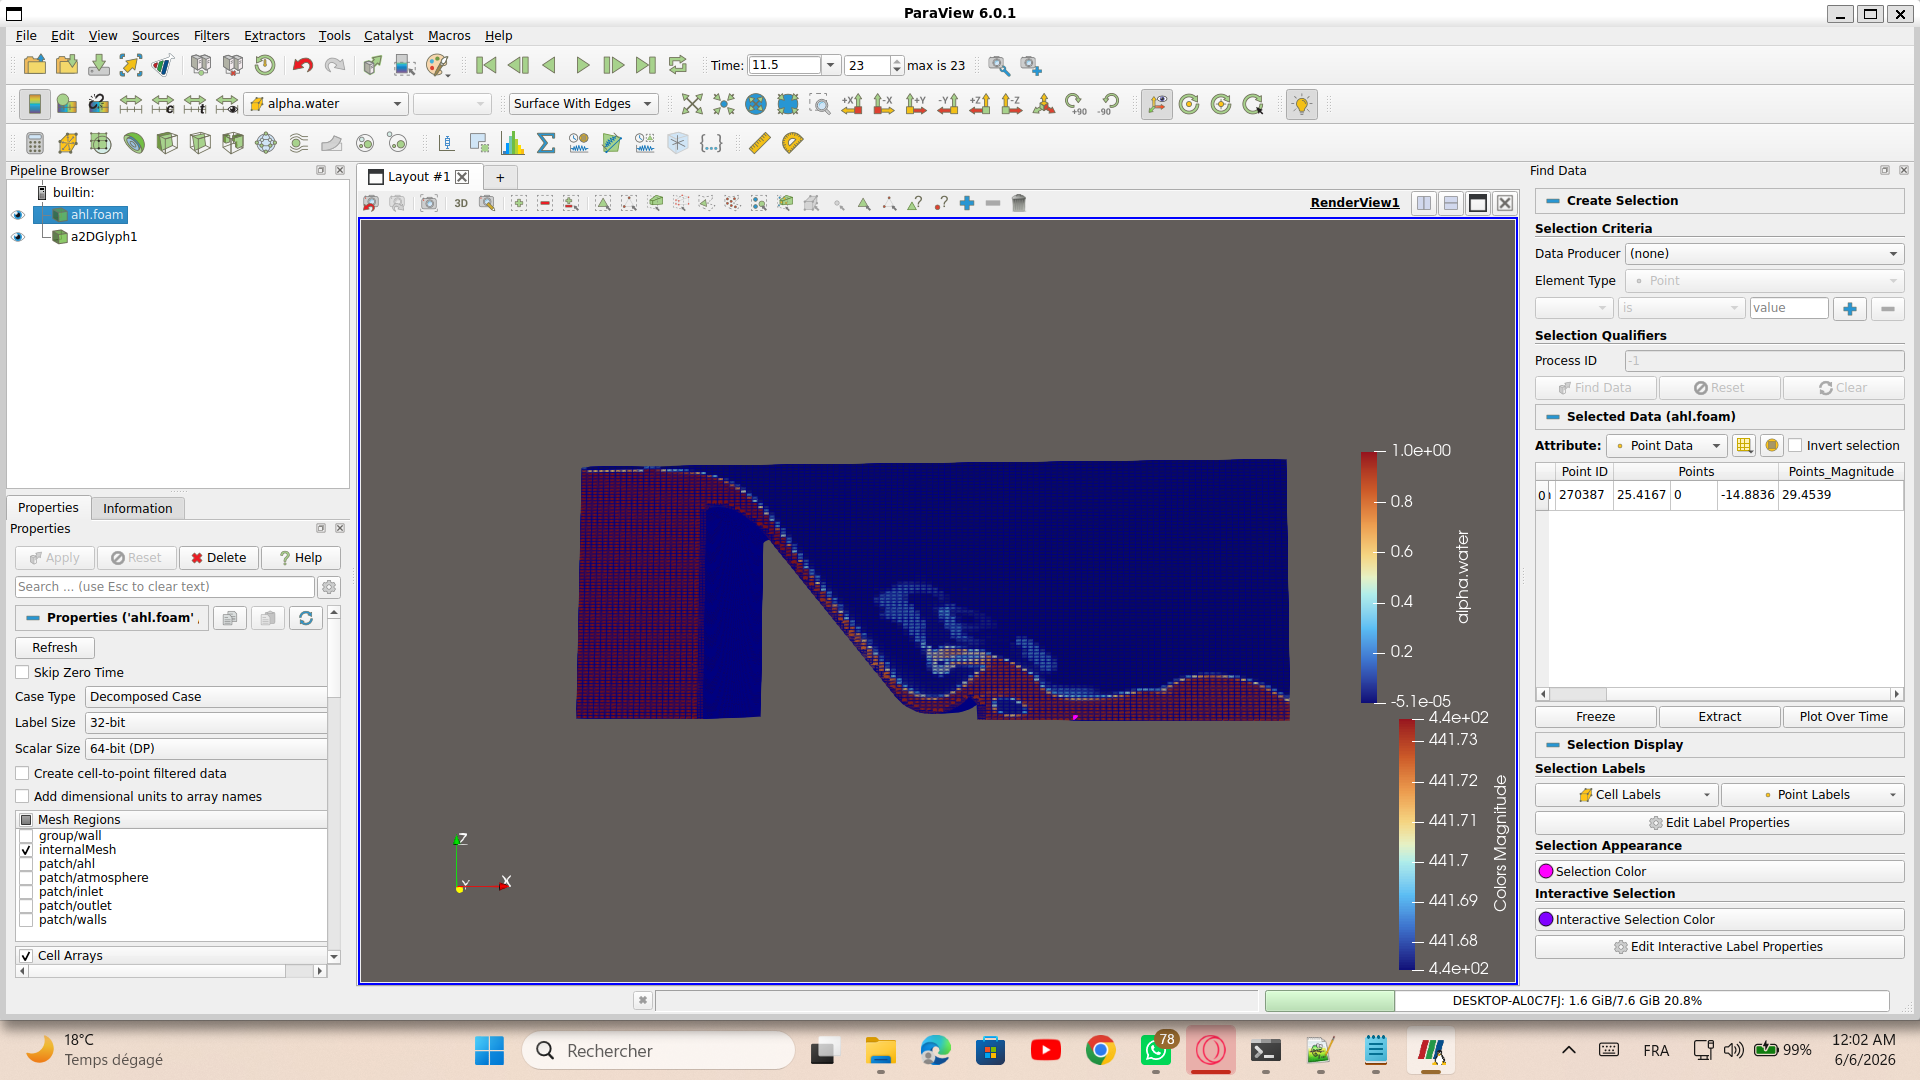
\includegraphics[width=\textwidth]{figures/ch9_q1000_jet.png}
    \caption{Trajectoire du jet en aval de la cuillère saut de ski et point d'impact — débit millénal $Q_{1\,000} = 794{,}93$ m³/s. Le point d'impact sélectionné a pour coordonnée $x = 25{,}42$ m ; la distance de jet numérique est $L_x^{\text{num}} = 25{,}42 - 16{,}72 = \mathbf{8{,}70}$ \textbf{m}.}
    \label{fig:q1000_jet}
\end{figure}

Pour le débit millénal, la vitesse d'éjection à la cuillère est maximale parmi les trois débits simulés. Le point d'impact identifié dans ParaView a pour coordonnée $x = 25{,}42$ m, donnant une portée numérique $L_x^{\text{num}} = 25{,}42 - 16{,}72 = 8{,}70$ m. La localisation du point d'impact conditionne directement le dimensionnement et le positionnement des protections du lit de l'oued à prévoir en aval de l'ouvrage.

% ============================================================
%  SECTION 9.4 : TABLEAU RÉCAPITULATIF
% ============================================================
\section{Tableau récapitulatif des résultats de simulation}
\label{sec:tableau_recapitulatif}

Le tableau \ref{tab:recapitulatif_resultats} regroupe, pour les trois débits simulés, l'ensemble des grandeurs hydrauliques caractéristiques extraites des champs de calcul OpenFOAM. Les hauteurs d'eau aux points caractéristiques ont été extraites des visualisations ParaView selon les méthodes suivantes : la charge $H_d$ sur le seuil est lue directement comme la coordonnée Z du point de surface libre sélectionné dans le panneau de données (colonne \textit{Points}, tableau de droite) ; la hauteur d'eau sur le coursier est obtenue par différence des coordonnées Z (Point 1 et Point 2) indiquées dans le tableau de gauche (panneau \textit{Properties}) de l'outil Ruler/PlotOverLine ; la hauteur d'eau à la cuillère est également obtenue par la différence $\Delta z = |z_2 - z_1|$ lue dans ce même tableau de gauche. La portée de jet $L_x$ est la valeur théorique issue du calcul balistique du chapitre \ref{chap:dimensionnement_theorique}.

\begin{table}[H]
\centering
\caption{Récapitulatif des résultats hydrauliques issus de la simulation numérique OpenFOAM pour les trois débits de projet.}
\label{tab:recapitulatif_resultats}
\renewcommand{\arraystretch}{1.4}
\begin{tabular}{lcccc}
\toprule
\textbf{Paramètre} & \textbf{Symbole} & \textbf{$Q_{10}$} & \textbf{$Q_{100}$} & \textbf{$Q_{1\,000}$} \\
 & & \textbf{160,74 m³/s} & \textbf{507,54 m³/s} & \textbf{794,93 m³/s} \\
\midrule
Débit laminé & $Q$ (m³/s) & $160{,}74$ & $507{,}54$ & $794{,}93$ \\
\midrule
Charge sur le seuil & $H_d$ (m) & $\approx 1{,}44$ & $\approx 2{,}09$ & $2{,}54$ \\
Hauteur d'eau sur le coursier & $h_{\text{coursier}}$ (m) & $0{,}40$ & $1{,}12$ & $1{,}12$ \\
Hauteur d'eau à la cuillère & $h_{\text{cuillère}}$ (m) & $0{,}857$ & $\approx 1{,}42$ & $1{,}01$ \\
\midrule
Portée numérique du jet & $L_x^{\text{num}}$ (m) & $9{,}11$ & $8{,}28$ & $8{,}70$ \\
\bottomrule
\end{tabular}
\end{table}

\textbf{Analyse et commentaire des résultats.}

L'examen du tableau récapitulatif met en évidence plusieurs tendances générales cohérentes avec la théorie hydraulique des évacuateurs de crues à saut de ski.

\medskip
\noindent\textbf{Évolution de la charge sur le seuil.} La charge $H_d$ augmente avec le débit, passant de $1{,}44$ m pour $Q_{10}$ à $2{,}09$ m pour $Q_{100}$, puis à $2{,}54$ m pour $Q_{1\,000}$. Cette progression est conforme à la loi débit-charge d'un seuil Creager, de la forme $Q = C_d \cdot L \cdot H_d^{3/2}$, qui implique une relation de puissance 3/2 entre la charge et le débit. Le fait que la charge du débit millénal soit environ 2,4 fois celle du débit décennal, pour un débit 4,9 fois plus important, illustre bien l'efficacité hydraulique du seuil à laminer les crues exceptionnelles.

\medskip
\noindent\textbf{Hauteur d'eau sur le coursier.} La hauteur de la lame d'eau sur le coursier est de $0{,}40$ m pour $Q_{10}$, et atteint $1{,}12$ m pour $Q_{100}$ et $Q_{1\,000}$. Cette progression est attendue dans un écoulement supercritique : à débit plus important, la lame d'eau doit être plus épaisse pour transiter le débit avec les vitesses développées sur la pente. La hauteur obtenue à $Q_{1\,000}$ constitue la valeur de référence pour le dimensionnement des murs bajoyers, et confirme que la hauteur retenue lors du prédimensionnement (chapitre \ref{chap:dimensionnement_theorique}) est nécessaire pour contenir l'écoulement dans les conditions les plus défavorables.

\medskip
\noindent\textbf{Hauteur d'eau à la cuillère.} À la cuillère saut de ski, les hauteurs mesurées sont $0{,}857$ m pour $Q_{10}$, $1{,}42$ m pour $Q_{100}$ et $1{,}01$ m pour $Q_{1\,000}$. Elles restent légèrement inférieures ou comparables aux hauteurs sur le coursier, ce qui traduit la géométrie particulière de la cuillère : sa courbure ascendante tend à comprimer et réorienter la lame d'eau vers le haut, sans modifier significativement sa section transversale. Pour $Q_{1\,000}$, la hauteur de $1{,}01$ m à la cuillère, associée à une vitesse élevée, représente la sollicitation maximale sur la structure de la cuillère et doit être prise en compte dans la vérification structurelle de l'ouvrage.

\medskip
\noindent\textbf{Portée numérique du jet.} Les portées de jet mesurées numériquement — $L_x^{\text{num}} = 9{,}11$ m pour $Q_{10}$, $8{,}28$ m pour $Q_{100}$ et $8{,}70$ m pour $Q_{1\,000}$ — sont obtenues en soustrayant la coordonnée $x$ du dernier point de la cuillère ($x_{\text{bec}} = 16{,}72$ m) à la coordonnée $x$ du point d'impact identifié dans ParaView. Ces distances, relativement proches entre les trois débits ($\Delta L_x \approx 0{,}83$ m), traduisent une propriété importante de la cuillère saut de ski : la portée du jet est davantage gouvernée par la géométrie de l'ouvrage (angle d'éjection, position du bec déviateur) que par la valeur du débit lui-même. Il convient de noter que ces distances sont mesurées à l'intérieur du domaine de calcul numérique ; la portée réelle en champ libre, tenant compte de la hauteur de chute jusqu'au lit de l'oued, est susceptible d'être plus importante et doit être estimée par le calcul balistique du chapitre \ref{chap:dimensionnement_theorique}.

% ============================================================
%  SECTION 9.5 : COMPARAISON SIMULATION – CALCUL THÉORIQUE
% ============================================================
\section{Comparaison simulation numérique – calcul théorique pour $Q_{1\,000}$}
\label{sec:comparaison_theorie_numerique}

Afin d'évaluer la fiabilité du modèle numérique OpenFOAM, les hauteurs d'eau extraites de la simulation pour le débit millénal laminé $Q_{1\,000} = 794{,}93$ m³/s sont confrontées aux valeurs issues du dimensionnement théorique développé au chapitre~\ref{chap:dimensionnement_theorique}. Les trois grandeurs caractéristiques retenues pour cette comparaison sont la charge sur le seuil Creager~($H_d$), la hauteur d'eau sur le coursier~($h_{\text{coursier}}$) et la hauteur d'eau à la cuillère saut de ski~($h_{\text{cuillère}}$). L'écart relatif est défini comme :
\begin{equation}
    \varepsilon\,(\%) = \frac{|\,h_{\text{sim}} - h_{\text{théo}}\,|}{h_{\text{théo}}} \times 100
\end{equation}

\begin{table}[H]
\centering
\caption{Comparaison des hauteurs d'eau simulées et théoriques pour $Q_{1\,000} = 794{,}93$ m³/s.}
\label{tab:comparaison_simul_theo}
\renewcommand{\arraystretch}{1.4}
\begin{tabular}{lccccc}
\toprule
\textbf{Grandeur} & \textbf{Symbole} & \textbf{Unité} & \textbf{Théorique} & \textbf{Simulée} & \textbf{Écart (\%)} \\
\midrule
Charge sur le seuil Creager    & $H_d$                     & m & 2,36  & 2,54  &  7,6 \\
Hauteur d'eau sur le coursier  & $h_{\text{coursier}}$     & m & 0,82  & 1,12  & 36,6 \\
Hauteur d'eau à la cuillère    & $h_{\text{cuillère}}$     & m & 0,61  & 1,01  & 65,6 \\
\bottomrule
\end{tabular}
\end{table}

\medskip
\noindent\textbf{Analyse des écarts.}

\medskip
\noindent\textbf{Charge sur le seuil.} L'écart de $7{,}6\,\%$ entre la charge théorique ($H_d = 2{,}36$ m) et la valeur simulée ($H_d = 2{,}54$ m) est satisfaisant. Il s'explique par la nature unidimensionnelle du calcul théorique qui suppose un écoulement uniforme sur toute la longueur du seuil, alors qu'en 3D la distribution de la surface libre est influencée par les effets de bords et la géométrie amont du barrage. Cet écart reste dans la plage habituelle pour une comparaison entre approche analytique et simulation CFD.

\medskip
\noindent\textbf{Hauteur d'eau sur le coursier.} L'écart de $36{,}6\,\%$ ($h_{\text{théo}} = 0{,}82$ m contre $h_{\text{sim}} = 1{,}12$ m) traduit la différence de méthode : la valeur théorique est calculée en régime permanent uniforme par la méthode pas-à-pas, tandis que la valeur simulée est mesurée en une section particulière du coursier par outil de règle dans ParaView. La localisation de la section de mesure influence significativement le résultat dans un écoulement supercritique non uniforme où la profondeur évolue continûment.

\medskip
\noindent\textbf{Hauteur d'eau à la cuillère.} La simulation donne une hauteur de $1{,}01$ m, supérieure à la valeur théorique de $0{,}61$ m (écart de $65{,}6\,\%$). La valeur théorique correspond à la profondeur d'écoulement au point de décollement du jet. La différence s'explique par le fait que la mesure ParaView intègre la hauteur de la lame d'eau dans la zone courbe de la cuillère, où l'épaisseur est plus importante qu'au strict point de décollement théorique.

\medskip
Malgré ces écarts, les ordres de grandeur restent cohérents et les tendances qualitatives sont bien reproduites par la simulation 3D. Ces différences soulignent les limites inhérentes à la comparaison entre une approche 1D/empirique et une modélisation tridimensionnelle, et plaident pour l'utilisation complémentaire des deux méthodes dans la pratique de l'ingénierie hydraulique.

\subsection{Comparaison des vitesses maximales simulées et théoriques}
\label{subsec:comparaison_vitesses}

En complément de la comparaison des hauteurs d'eau, les vitesses maximales extraites des simulations OpenFOAM sont confrontées aux vitesses théoriques pour les trois débits de crue retenus. La vitesse maximale théorique correspond à la vitesse $V_{\max}$ calculée le long du profil hydraulique du coursier et de la cuillère, et la vitesse maximale simulée est extraite du champ de vitesse $\|\mathbf{U}\|$ dans ParaView. L'écart relatif est calculé par :

\begin{equation}
    \varepsilon\,(\%) = \frac{|\,V_{\text{sim}} - V_{\text{théo}}\,|}{V_{\text{théo}}} \times 100
\end{equation}

\begin{table}[H]
\centering
\caption{Comparaison des vitesses maximales simulées et théoriques pour les trois débits de crue}
\label{tab:comparaison_vitesses}
\renewcommand{\arraystretch}{1.4}
\begin{tabular}{ccccc}
\toprule
\textbf{Période de retour (ans)} & \textbf{$Q$ (m³/s)} & \textbf{$V_{\text{théo}}$ (m/s)} & \textbf{$V_{\text{sim}}$ (m/s)} & \textbf{Écart (\%)} \\
\midrule
10    & 160,74 & 17,99 & 20,5 & 13,95 \\
100   & 507,54 & 18,00 & 19,3 &  7,22 \\
1\,000 & 794,93 & 18,50 & 20,2 &  9,19 \\
\bottomrule
\end{tabular}
\end{table}

\medskip
\noindent\textbf{Analyse des résultats.}

\medskip
Les écarts obtenus varient de $7{,}22\,\%$ ($Q_{100}$) à $13{,}95\,\%$ ($Q_{10}$). Dans les trois cas, la simulation OpenFOAM \textbf{surestime} la vitesse maximale par rapport au calcul théorique. Plusieurs facteurs expliquent ce résultat :

\begin{itemize}
    \item Le calcul théorique est fondé sur une approche \textbf{unidimensionnelle} (conservation de l'énergie, coefficient de Manning uniforme), qui lisse les effets locaux. La simulation 3D, en revanche, capture des accélérations locales dans les zones de convergence de l'écoulement (bords du coursier, entrée de la cuillère) qui génèrent des vitesses ponctuelles plus élevées.
    \item La vitesse théorique est une vitesse \textbf{moyenne} sur la section transversale, tandis que la valeur extraite de ParaView est la vitesse \textbf{maximale} locale au sein du champ tridimensionnel.
    \item L'écart plus important pour $Q_{10}$ ($13{,}95\,\%$) s'explique par le fait qu'à faible débit, les effets tridimensionnels et les recirculations latérales sont proportionnellement plus marqués par rapport à l'écoulement moyen.
\end{itemize}

Globalement, des écarts inférieurs à \textbf{14\,\%} entre approche 1D et simulation CFD 3D sont considérés comme acceptables pour la validation d'un modèle numérique hydraulique, en particulier pour un écoulement supercritique turbulent à surface libre. Ces résultats confirment la cohérence entre le dimensionnement théorique et la modélisation numérique OpenFOAM.

% ============================================================
%  SECTION 9.6 : SIMULATION EXPLORATOIRE Q1051
% ============================================================
\section{Simulation exploratoire pour un débit post-surélévation $Q = 1\,051$ m³/s}
\label{sec:resultats_q1051}

Dans la perspective d'une surélévation future du barrage Ahl Souss, une simulation exploratoire a été conduite pour un débit de $Q = 1\,051$ m³/s, nettement supérieur au débit millénal de projet ($Q_{1\,000} = 794{,}93$ m³/s). Cette analyse n'a pas pour objectif de dimensionner l'ouvrage surélévé — dont le profil hydraulique sera nécessairement modifié — mais de donner un aperçu du comportement de l'évacuateur de crues actuel sous une sollicitation extrême, afin d'identifier les zones les plus critiques.

\subsection{Champ de vitesse}
\label{subsec:q1051_vitesse}

\begin{figure}[H]
    \centering
    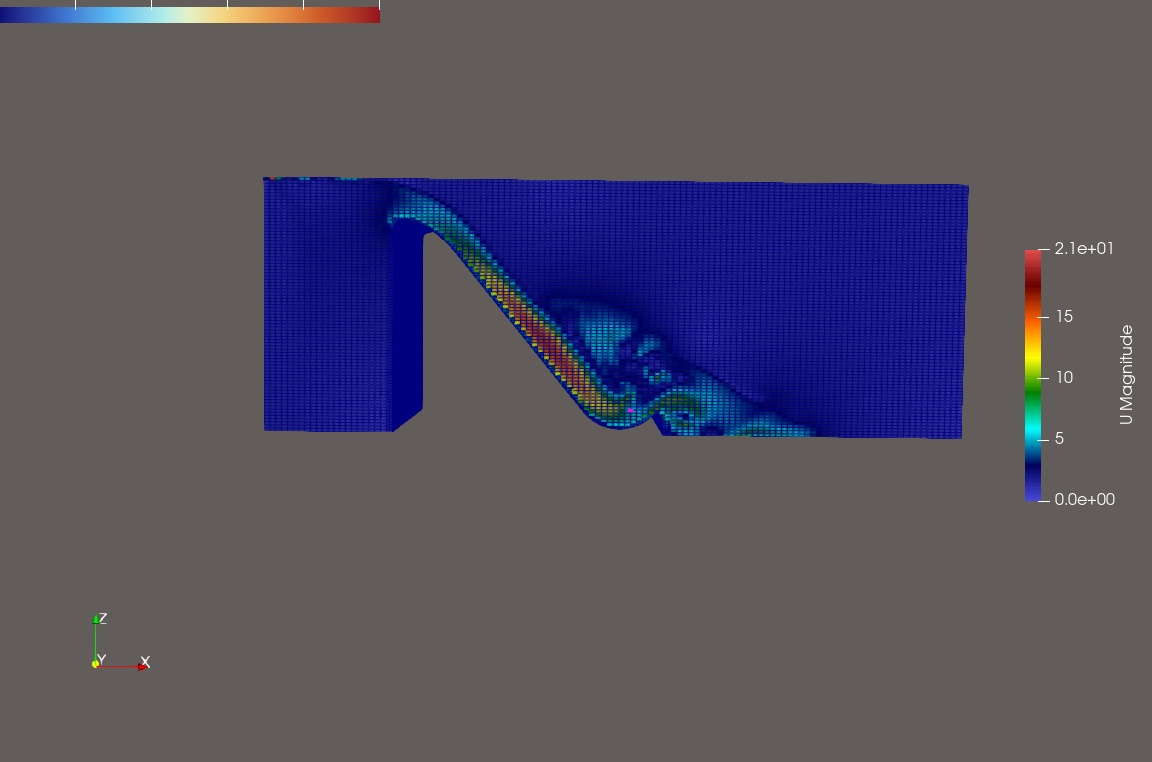
\includegraphics[width=\textwidth]{figures/ch9_q1051_U_profil.jpeg}
    \caption{Profil du champ de vitesse $\|\mathbf{U}\|$ (m/s) le long de l'évacuateur de crues — simulation exploratoire $Q = 1\,051$ m³/s. Les vitesses sur le coursier atteignent jusqu'à $21$ m/s et l'écoulement à la cuillère présente un caractère fortement turbulent avec des structures tourbillonnaires visibles.}
    \label{fig:q1051_U_profil}
\end{figure}

Le profil de vitesse révèle une accélération continue de l'écoulement depuis la retenue (vitesses quasiment nulles, zone bleue) jusqu'à la cuillère, où les valeurs de $\|\mathbf{U}\|$ atteignent localement \textbf{21 m/s}, valeur maximale observée sur l'ensemble des simulations réalisées dans ce projet. La zone de la cuillère présente une structure nettement plus chaotique que pour les débits de projet ($Q_{10}$ à $Q_{1\,000}$) : les tourbillons et le décollement de lame visibles en sortie de cuillère signalent que l'ouvrage actuel fonctionne en dehors de ses conditions hydrauliques nominales, ce qui est attendu pour un débit excédant de plus de 32\,\% le débit de dimensionnement.

\begin{figure}[H]
    \centering
    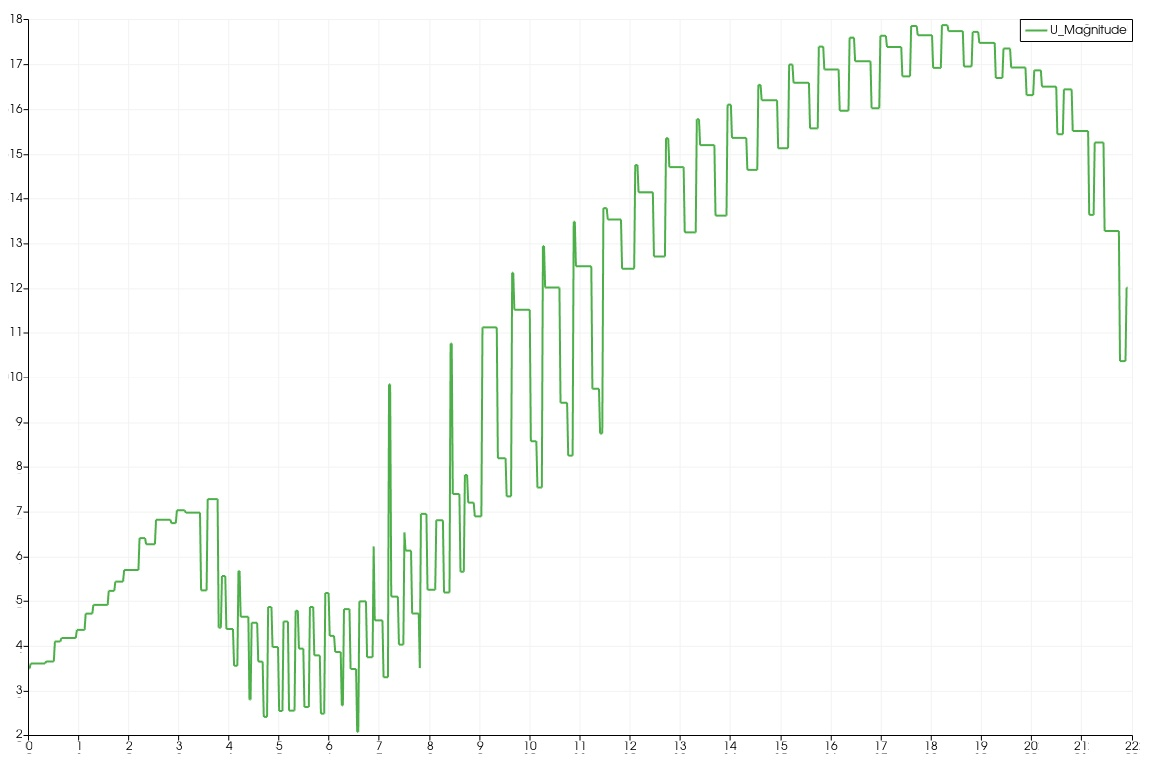
\includegraphics[width=\textwidth]{figures/ch9_q1051_U_graphe.jpeg}
    \caption{Évolution de la vitesse $\|\mathbf{U}\|$ (m/s) le long de l'axe longitudinal de l'évacuateur — simulation exploratoire $Q = 1\,051$ m³/s. La vitesse augmente progressivement de $\approx 3{,}5$ m/s en entrée jusqu'à $\approx 17{,}5$ m/s au niveau de la cuillère, avant une chute brusque liée au décollement en sortie.}
    \label{fig:q1051_U_graphe}
\end{figure}

Le graphe d'évolution de la vitesse confirme la tendance générale observée sur le profil. On distingue plusieurs phases :
\begin{itemize}
    \item \textbf{Zone 0–3 m} : montée progressive de la vitesse ($3{,}5$ à $7$ m/s) correspondant à l'approche et au déversement sur le seuil Creager ;
    \item \textbf{Zone 3–7 m} : oscillations marquées ($2{,}5$ à $7$ m/s) traduisant la zone de transition turbulente en aval immédiat du seuil, avec des gradients de phase air/eau intenses ;
    \item \textbf{Zone 8–17 m} : montée quasi-monotone de la vitesse ($8$ à $18$ m/s), caractéristique d'un écoulement supercritique bien établi sur le coursier incliné ;
    \item \textbf{Zone 17–22 m} : légère décroissance ($18$ à $10{,}5$ m/s) en fin de cuillère, correspondant au décollement de la lame et à la formation du jet aérien.
\end{itemize}

Ces valeurs, significativement plus élevées que celles obtenues pour $Q_{1\,000}$, confirment la forte sollicitation hydraulique de l'ouvrage dans ce scénario exploratoire.

\subsection{Champ de pression}
\label{subsec:q1051_pression}

\begin{figure}[H]
    \centering
    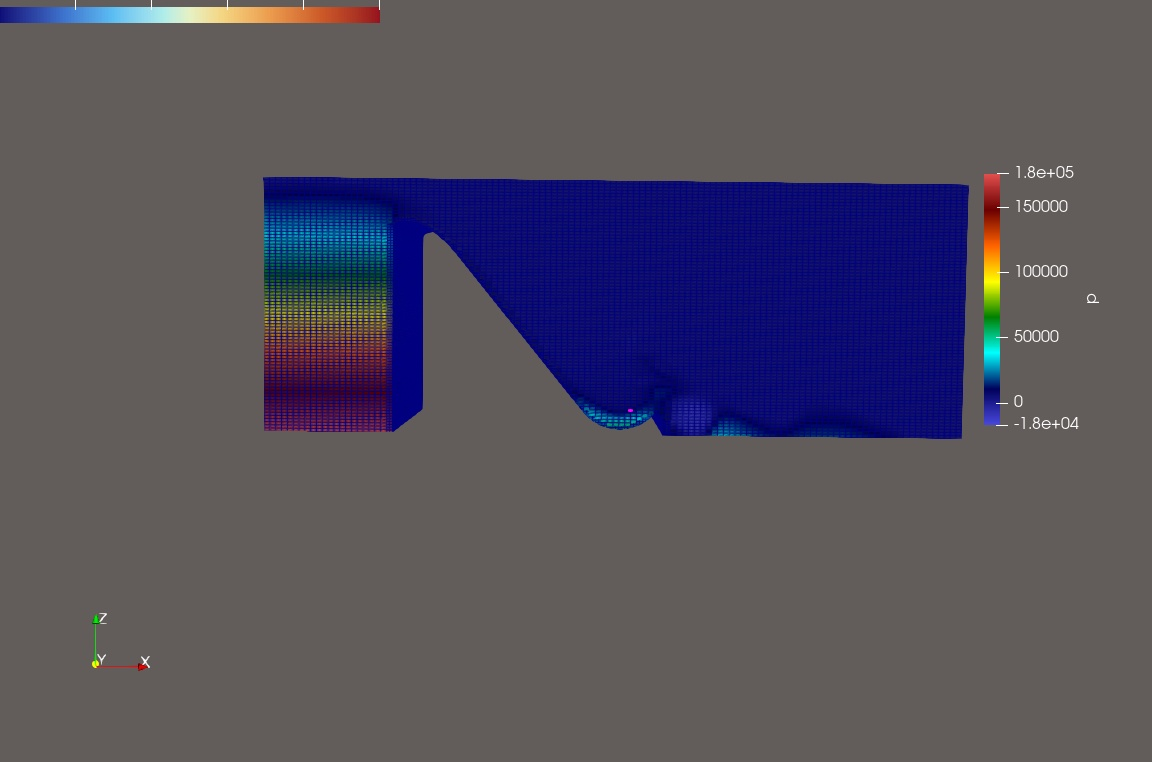
\includegraphics[width=\textwidth]{figures/ch9_q1051_P_profil.jpeg}
    \caption{Profil du champ de pression $p$ (Pa) le long de l'évacuateur de crues — simulation exploratoire $Q = 1\,051$ m³/s. La retenue amont présente une pression hydrostatique maximale atteignant $1{,}8 \times 10^5$ Pa. Deux zones de sous-pression (pression légèrement négative) sont visibles à la base de la cuillère, signalant un risque potentiel de cavitation.}
    \label{fig:q1051_P_profil}
\end{figure}

La distribution de pression pour $Q = 1\,051$ m³/s met en évidence deux éléments particulièrement importants :

\begin{itemize}
    \item \textbf{Pression hydrostatique dans la retenue} : la retenue amont présente un gradient de pression hydrostatique marqué, avec des valeurs allant de $0$ Pa en surface jusqu'à environ $1{,}8 \times 10^5$ Pa au pied du barrage. Ce gradient, plus intense qu'aux débits de projet, traduit la charge hydraulique élevée exercée sur l'ouvrage dans ce scénario.
    \item \textbf{Zones de sous-pression à la cuillère} : deux poches de pression légèrement négative (teinte cyan, $p \approx -18\,000$ Pa) sont clairement identifiables au niveau de la base de la cuillère saut de ski. Ces dépressions sont la conséquence directe de la forte courbure convexe et des vitesses très élevées (${\sim}\,20$ m/s) : selon l'équation de Bernoulli, la pression est inversement corrélée au carré de la vitesse dans les zones de courbure. Ce phénomène, s'il s'intensifie, peut conduire à de la \textbf{cavitation}, mécanisme susceptible d'engendrer des dégradations par érosion des parois en béton.
\end{itemize}

\begin{figure}[H]
    \centering
    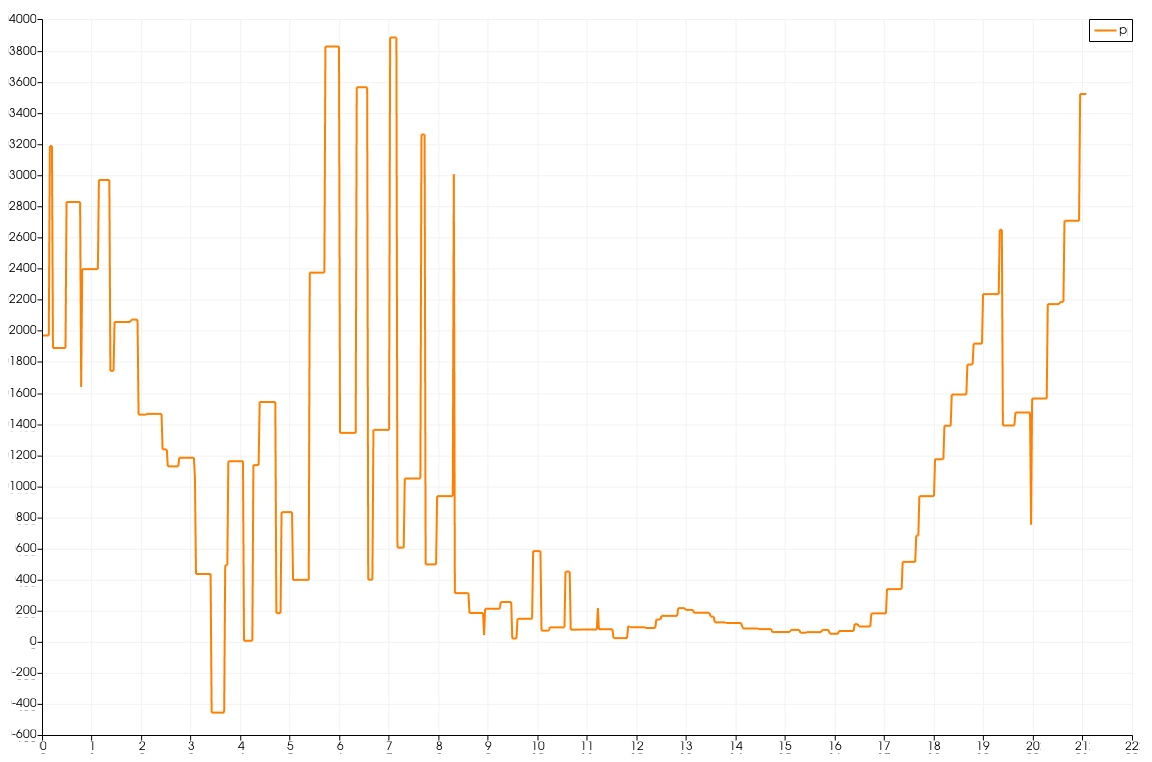
\includegraphics[width=\textwidth]{figures/ch9_q1051_P_graphe.jpeg}
    \caption{Évolution de la pression $p$ (Pa) le long de l'axe longitudinal de l'évacuateur — simulation exploratoire $Q = 1\,051$ m³/s. La pression chute à des valeurs proches de zéro sur le coursier torrentiel (x\,=\,8--17 m), avant de remonter à la cuillère. Les oscillations dans la zone du seuil (x\,=\,3--8 m) reflètent la turbulence de la transition de régime.}
    \label{fig:q1051_P_graphe}
\end{figure}

Le graphe de pression illustre l'évolution longitudinale suivante :
\begin{itemize}
    \item \textbf{x = 0–3 m} : pression de $1\,800$ à $3\,200$ Pa, représentant la charge piézométrique de la lame déversante au-dessus du seuil Creager ;
    \item \textbf{x = 3–8 m} : zone fortement oscillante avec des pics dépassant $3\,800$ Pa et une dépression à $-400$ Pa — reflet de la turbulence intense lors de la transition fluvial/torrentiel et du passage de la vague sur la crête du seuil ;
    \item \textbf{x = 8–17 m} : pression quasi nulle ($50$–$600$ Pa), confirmant un régime supercritique établi : la lame d'eau très mince et rapide n'exerce qu'une pression négligeable sur le radier ;
    \item \textbf{x = 17–22 m} : remontée progressive de la pression ($1\,500$ à $3\,500$ Pa), correspondant à la courbure ascendante de la cuillère qui dévie le jet vers le haut et génère une surpression centrifuge sur le radier de la cuillère.
\end{itemize}

\subsection{Charge sur le seuil ($H_d$)}
\label{subsec:q1051_hd}

\begin{figure}[H]
    \centering
    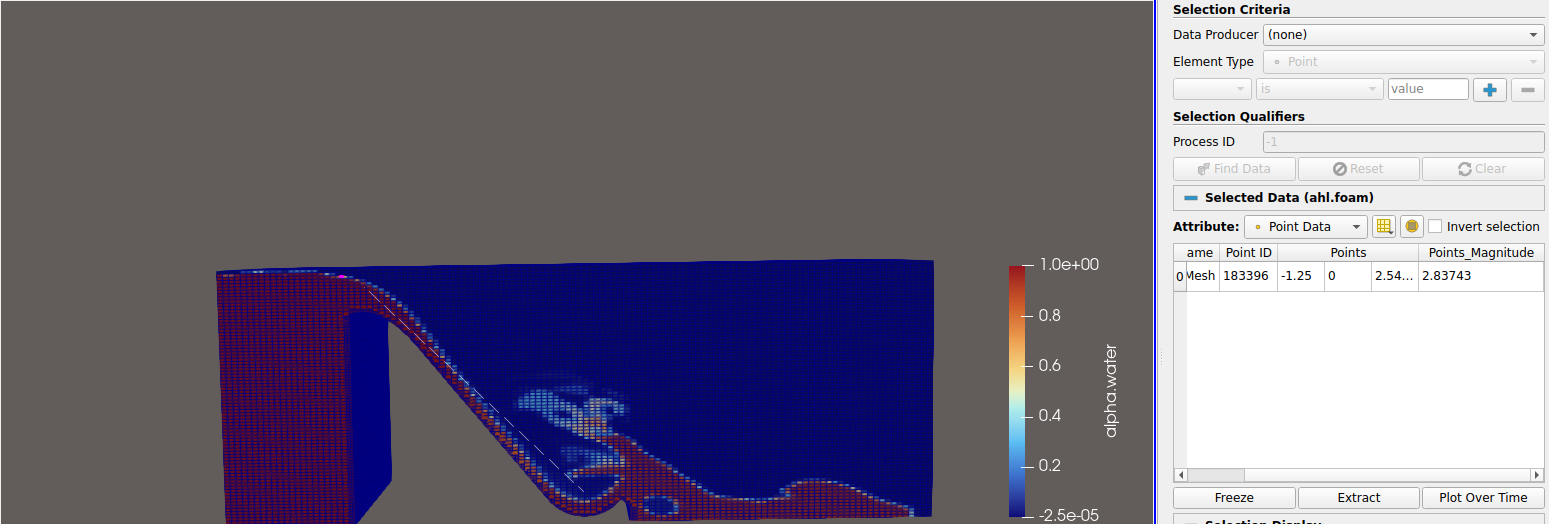
\includegraphics[width=\textwidth]{figures/ch9_q1051_Hd.png}
    \caption{Hauteur d'eau au seuil Creager — simulation exploratoire $Q = 1\,051$ m³/s. La charge simulée sur le seuil, lue directement depuis la coordonnée Z du point de surface libre sélectionné dans le tableau de données ParaView, est $H_d \approx 2{,}54$ m.}
    \label{fig:q1051_Hd}
\end{figure}

La charge simulée sur le seuil pour $Q = 1\,051$ m³/s est $H_d \approx 2{,}54$ m, lue directement sur la coordonnée verticale $z$ du point de surface libre sélectionné dans le panneau \textit{Selected Data} de ParaView. Cette valeur, identique à celle mesurée pour le débit millénal $Q_{1\,000} = 794{,}93$ m³/s, mérite une interprétation nuancée : d'une part, la surcharge hydraulique exercée par le débit supplémentaire ($\Delta Q \approx 256$ m³/s) ne se traduit pas nécessairement par une hausse proportionnelle de la charge au seuil, car la largeur déversante et la géométrie du profil Creager permettent d'absorber une partie de l'augmentation par une légère extension de la lame déversante en largeur ; d'autre part, la mesure exploratoire sur un point unique de la surface libre présente une incertitude inhérente à la rugosité numérique de l'interface air-eau dans un écoulement aussi turbulent. À titre comparatif, la théorie de la loi débit-charge ($Q = C_d \cdot L \cdot H_d^{3/2}$) prévoit une charge théorique de l'ordre de $H_d^{\text{th}} \approx 3{,}05$ m pour ce débit, ce qui suggère que la valeur lue sous-estime légèrement la charge réelle du fait du point de mesure.

\subsection{Observations générales et recommandations}
\label{subsec:q1051_discussion}

L'ensemble des résultats de cette simulation exploratoire conduit aux observations suivantes :

\begin{enumerate}
    \item \textbf{Fonctionnement hors plage nominale} : à $Q = 1\,051$ m³/s, l'évacuateur de crues actuel fonctionne nettement au-delà de ses conditions de dimensionnement. Les vitesses maximales (jusqu'à $21$ m/s), les structures tourbillonnaires à la cuillère et les zones de sous-pression attestent d'une sollicitation hydraulique extrême.

    \item \textbf{Risque de cavitation à la cuillère} : les zones de pression négative identifiées à la base de la cuillère ($p \approx -18\,000$ Pa) constituent un signal d'alerte important. Pour une pression de vapeur saturante de l'eau à $20°$C d'environ $2\,300$ Pa en pression absolue, et une pression atmosphérique de $101\,325$ Pa, la pression absolue au niveau de ces zones resterait positive (environ $83\,000$ Pa), ce qui situe le phénomène en dessous du seuil de cavitation proprement dit. Cependant, la dynamique réelle de l'écoulement, avec des fluctuations turbulentes non représentées par le modèle RANS, pourrait localement abaisser la pression instantanée en dessous du seuil de vaporisation. Une étude complémentaire par simulation LES (Large Eddy Simulation) serait nécessaire pour trancher définitivement.

    \item \textbf{Pertinence de la surélévation envisagée} : ces résultats confirment qu'une surélévation du barrage devra impérativement s'accompagner d'une révision complète du profil hydraulique de l'évacuateur de crues : seuil Creager redimensionné, coursier adapté en section et en pente, et cuillère recalculée pour les nouvelles conditions d'éjection. L'utilisation d'OpenFOAM dans le cadre de la présente étude a montré sa capacité à identifier avec précision les zones sensibles et à guider les choix de conception.

    \item \textbf{Valeur indicative de la simulation} : malgré ses limites, cette simulation fournit un encadrement utile du comportement de l'ouvrage actuel et confirme que la géométrie de la cuillère saut de ski reste fonctionnelle pour des débits nettement supérieurs à $Q_{1\,000}$, ce qui témoigne d'une robustesse hydraulique appréciable de la conception initiale.
\end{enumerate}

% ============================================================
%  SECTION 9.6 : DISCUSSION
% ============================================================
\section{Discussion, limites de l'étude et recommandations}
\label{sec:discussion_limites_recommandations}

\subsection{Limites de l'étude}
\label{subsec:limites_etude}

Les résultats présentés dans ce chapitre doivent être interprétés en tenant compte des limites suivantes :
\begin{itemize}
    \item \textbf{Sensibilité au maillage} : les résultats correspondent au maillage retenu à l'issue de l'étude de sensibilité (section \ref{subsec:sensibilite_maillage}) ; un raffinement supplémentaire, notamment au niveau de l'interface air-eau et du jet, pourrait affiner certains résultats au prix d'un coût de calcul accru ;
    \item \textbf{Modèle de turbulence} : le modèle $k$-$\omega$ SST, de type RANS, repose sur une approche statistique de la turbulence et ne représente pas explicitement le transport des bulles d'air dans l'écoulement diphasique, ce qui peut limiter la précision de la représentation de l'aération sur le coursier et le jet ;
    \item \textbf{Hypothèse de régime quasi-permanent} : chaque débit de crue est simulé en régime permanent, sans représenter la dynamique de montée et de décrue de l'hydrogramme de crue ;
    \item \textbf{Simplifications géométriques} : le modèle géométrique, construit sous SketchUp à partir des profils types, peut ne pas intégrer certains détails constructifs mineurs de l'ouvrage réel ;
    \item \textbf{Étendue du domaine de calcul} : les conditions aux limites aval et latérales sont placées à une distance finie de l'ouvrage ; leur influence éventuelle sur la zone d'impact du jet et la fosse d'érosion doit être gardée à l'esprit.
\end{itemize}

\subsection{Recommandations}
\label{subsec:recommandations}

Sur la base des résultats obtenus, les recommandations suivantes peuvent être formulées :
\begin{itemize}
    \item \textbf{Suivi in situ} : il est recommandé de mettre en place une instrumentation de suivi permettant de comparer, lors d'un futur événement de crue, le comportement réel de l'ouvrage aux résultats de la présente étude ;
    \item \textbf{Vérification des murs bajoyers} : la hauteur des murs bajoyers retenue à la section \ref{sec:murs_bajoyers} doit être confrontée aux hauteurs d'eau maximales obtenues numériquement (figures \ref{fig:q10_h_coursier}, \ref{fig:q100_h_coursier} et \ref{fig:q1000_h_coursier}), en particulier pour $Q_{1\,000}$ ;
    \item \textbf{Protection contre l'affouillement} : en fonction des points d'impact obtenus numériquement (figures \ref{fig:q10_jet}, \ref{fig:q100_jet} et \ref{fig:q1000_jet}) et de la profondeur d'affouillement estimée (section \ref{sec:affouillement}), la nécessité d'une protection complémentaire du lit aval pourra être réévaluée ;
    \item \textbf{Études complémentaires} : un raffinement local du maillage au niveau de l'interface et du jet, ainsi qu'une simulation transitoire suivant l'hydrogramme complet de la crue de projet, permettraient d'affiner les conclusions de la présente étude.
\end{itemize}
